% \begin{filecontents*}{\jobname.xmpdata}
%     \Title{Context Pruning for More Robust SMT-based Program Verification}
%     \Author{Yi Zhou\sep Jay Bosamiya\sep Jessica Li\sep Marijn \sep Bryan Parno}
%     \Publisher{TU Wien Academic Press}
%   \end{filecontents*}
  
  \PassOptionsToPackage{dvipsnames}{xcolor}
  \documentclass[year=25,pdfa]{fmcad}
  
  \usepackage{cite}
  \usepackage{amsmath,amssymb,amsfonts,amsthm}
  % \usepackage{algorithmic}
  \usepackage{graphicx}
  \usepackage{textcomp}
  \usepackage[dvipsnames]{xcolor}
  \usepackage{bussproofs}  % For natural deduction proofs with \inferrule
  \usepackage{mathpartir}
  \usepackage{orcidlink}
  \usepackage{booktabs}
  \usepackage{siunitx}
  % \usepackage{appendix}

  
  % \usepackage[margin=1in]{geometry}    % Exert more control over the margins
  % \usepackage{mathptm}     % Puts math text into the postscript Times font and symbol font (else uses the metafont-generated characters)
  % \usepackage{amsmath}     % Provides various features to facilitate writing math formulae and to improve the typographical quality of their output
  \usepackage{float}       % Basic package for floating objects like figures and tables
  % \usepackage{psfrag}      % Used to insert text into figures
  % \usepackage{floatflt}    % Used to wrap text around figures
  % \usepackage{graphicx}    % Used to display graphic figures and such
  \usepackage{xspace}      % Intelligently adds space after a word via \xspace
  % \usepackage{color}       % Used to highlight comments
  % \usepackage{pifont}      % Provides the ding symbol used for comments
  % \usepackage{subfigure}   % Place two related figures side-by-side
  % \usepackage{url}         % Properly formats URLs
  % \usepackage{array}       % Add more space to the tables
  % \usepackage{algorithm}   % Defines algorithm float environment
  % \usepackage{algpseudocode}
  \usepackage{multirow}    % Use to create table with a column that spans multiple rows
  \usepackage{enumerate}   % Control the numbering for enumerated lists
  \usepackage[square,comma,numbers,sort&compress]{natbib}      % Offers more control over citation appearance and bib spacing
  % \usepackage{enumitem}
  \usepackage{diagbox}
  % \usepackage{makecell}
  \usepackage{booktabs}
  % \usepackage[T1]{fontenc}
  \usepackage[noend]{algpseudocode}
  % \usepackage{algpseudocode}
  % \usepackage{authblk}
  \usepackage{pifont}
  % \usepackage[switch]{lineno} % Line numbering for draft-mode
  % \usepackage{tikz}
  % \usetikzlibrary{shapes.geometric, arrows}
  % \usetikzlibrary{decorations.pathreplacing,calligraphy}
  \usepackage{tikz}
  \usetikzlibrary{matrix}

  % ------------------------------------------------------------------
  % Dot grid styles 
  \newcommand*\dotdiam{15pt}      % <— tweak this for bigger / smaller circles
  \newcommand*\dotgap {4pt}      % <— negative → dots touch; 0pt = tangent

  \tikzset{
    cell/.style   = {draw,circle,fill=gray!60,
                    minimum size=\dotdiam, inner sep=0pt, outer sep=0pt,
                    text height=1.5ex, text depth=0.5ex},
    redcell/.style= {cell,fill=red!60},
    redpluscell/.style= {cell,fill=red!60,execute at begin node={\Large +}},
    redminuscell/.style= {cell,fill=red!60,execute at begin node={\Large -}},
    greencell/.style  = {cell,fill=green!60},
    greenpluscell/.style  = {cell,fill=green!60,execute at begin node={\Large +}},
    greenminuscell/.style  = {cell,fill=green!60,execute at begin node={\Large -}},
    graycell/.style = {cell,fill=gray!40},
    graypluscell/.style = {cell,fill=gray!40,execute at begin node={\Large +}},
    grayminuscell/.style = {cell,fill=gray!40,execute at begin node={\Large -}},
    bluecell/.style = {cell,fill=blue!20},
    bluepluscell/.style = {cell,fill=blue!20,execute at begin node={\Large +}},
    blueminuscell/.style = {cell,fill=blue!20,execute at begin node={\Large -}},
    yellowcell/.style = {cell,fill=yellow!60},
    yellowpluscell/.style = {cell,fill=yellow!60,execute at begin node={\Large +}},
    yellowminuscell/.style = {cell,fill=yellow!60,execute at begin node={\Large -}},
    purplecell/.style = {cell,fill=purple!60},
    purplepluscell/.style = {cell,fill=purple!60,execute at begin node={\Large +}},
    purpleminuscell/.style = {cell,fill=purple!60,execute at begin node={\Large -}},
    orangecell/.style = {cell,fill=orange!60},
    orangepluscell/.style = {cell,fill=orange!60,execute at begin node={\Large +}},
    orangeminuscell/.style = {cell,fill=orange!60,execute at begin node={\Large -}},
    gridmatrix/.style = {
        matrix of nodes,
        nodes   = {cell},
        column sep=\dotgap, row sep=\dotgap,
        % ampersand replacement=\&,                      % enable & inside matrix
        nodes in empty cells,                          % draw every entry
    },
  }
  \usepackage{subcaption}
  
% }
  \usepackage{outlines}
  \usepackage{listings}
  % \usepackage[caption=false]{subfig}
  \usepackage{soul}
  \usepackage{microtype}
  
  \def\BibTeX{{\rm B\kern-.05em{\sc i\kern-.025em b}\kern-.08em
      T\kern-.1667em\lower.7ex\hbox{E}\kern-.125emX}}
  
  % Used for displaying a sample figure. If possible, figure files should
  % be included in EPS format.
  %
  % If you use the hyperref package, please uncomment the following line
  % to display URLs in blue roman font according to Springer's eBook style:
  % \renewcommand\UrlFont{\color{blue}\rmfamily}
  
  
  \usepackage[linesnumbered,ruled,vlined]{algorithm2e}
  % \SetAlCapSkip{1em} % or 10pt, 12pt, etc.
  \usepackage{hyperref}
  \hypersetup{
  %\ifpdf
  %        pdftex,
  %\else
  %        dvipdf,
  %\fi
    %pdftex,              % using ps2pdf vs pdftex
    %ps2pdf,              % using ps2pdf vs pdftex
          %hypertex,
    colorlinks=true,     % color the words instead of use a colored box
    urlcolor=blue,       % \href{...}{...} external (URL)
  %  filecolor=blue,      % \href{...} local file
    linkcolor=blue,     % \ref{...} and \pageref{...}
    citecolor=blue,     % \cite{}
  % letterpaper=true,
    plainpages=false,
  %    plainpages          boolean         true
  %    Forces page anchors to be named by the arabic form of the page number,
  %    rather than the formatted form.
    breaklinks=true,
  %    breaklinks          boolean         false
  %    Allows link text to break across lines; since this cannot be accommodated in
  %    PDF, it is only set true by default if the pdftex driver is used. This makes
  %    links on multiple lines into different PDF links to the same target.
  % pagebackref=true,
  %     Adds ?backlink? text to the end of each item in the bibliography, as a list
  %     of section numbers. This can only work properly if there is a blank line
  %     after each \bibitem.
    bookmarksnumbered=true,
  %    bookmarksnumbered   boolean         false
  %    If Acrobat bookmarks are requested, include section numbers.
    bookmarksopen=true,
  %    bookmarksopen       boolean         false
  %    If Acrobat bookmarks are requested, show them with all the subtrees expanded.
    pdftitle={},
    pdfauthor={},
    pdfkeywords={},
  % pdfpagelabels=true,
    pdfpagemode=UseOutlines  % None, UseThumbs, UseOutlines, FullScreen
  }

  \renewcommand{\sectionautorefname}{Section}
  \renewcommand{\subsectionautorefname}{Subsection}
  \renewcommand{\algorithmautorefname}{Algorithm}


  
  \usepackage[capitalise]{cleveref}
%   \usepackage{stys/dafny}
%   \usepackage{stys/smtlib}
  % \usepackage{array}
  \usepackage{tabularx}
  
%   \input{00-common-preamble.tex}
  
  % \algrenewcommand\algorithmicindent{0.65em}%

  \newtheorem{definition}{Definition}
  \newtheorem{theorem}{Theorem}
  \newtheorem{lemma}{Lemma}
  \newtheorem{claim}{Claim}


  
  \newcommand{\unsat}{\texttt{unsat}\xspace}
  \newcommand{\sat}{\texttt{sat}\xspace}
  \newcommand{\tool}{CA\textsc{uti}C\textsc{aL}\xspace}
  \newcommand{\toolminus}{$\text{CA}\textsc{uti}\text{C}\textsc{aL}^{-}$\xspace}
  \newcommand{\pr}{\textsf{PR}\xspace}
  \newcommand{\er}{\texttt{ER}\xspace}
  \newcommand{\impunit}{\vdash_1}
  \newcommand{\impunitclause}[3]{#1 \land \overline{#2} \impunit #3}
  \newcommand{\lingeling}{\textsc{lingeling}\xspace}
%  \newcommand{\cadical}{{\sf CaDiCaL}\xspace}
  \newcommand{\cadical}{C\textsc{a}D\textsc{i}C\textsc{aL}\xspace}
  \newcommand{\sadical}{S\textsc{a}D\textsc{i}C\textsc{aL}\xspace}
  \newcommand{\glucoser}{G\textsc{lucos}ER\xspace}
  \newcommand{\prelearn}{PR\textsc{e}L\textsc{earn}\xspace}
  \newcommand{\ph}[1]{\ensuremath{\mathrm{PHP}(#1)}}
  
    \newcommand{\kissat}{\textsc{Kissat}\xspace}
    \newcommand{\cryptoMiniSAT}{\textsc{CryptoMiniSAT}\xspace}


  \newcommand{\impunitclause}[3]{$#1 \impunit #2 \lor #3$} 
  
  \begin{document}
  \title{Learning Short Clauses via Conditional Autarkies}
  
  % \author{TODO: add authors and orcid \\
  \author{Amar Shah \orcidlink{0009-0008-8282-2142}, Twain Byrnes \orcidlink{0009-0000-7939-1195}, Joseph Reeves \orcidlink{0000-0002-4585-0565}, Marijn J.\ H.\ Heule \orcidlink{0000-0002-5587-8801} \\
  \emph{Carnegie Mellon University, Pittsburgh, PA, USA} \\
  \texttt{\small amarshah@cmu.edu, binarynewts@cmu.edu, jereeves@andrew.cmu.edu, marijn@cmu.edu}}
  
  \maketitle
  
  \begin{abstract}
    % \input{texs/abstract}
    State-of-the-art Boolean satisfiability (SAT) solvers increasingly use techniques beyond resolution.
    One of the strongest such techniques is Propagation Redundancy (PR) learning.
    %
    Solvers utilizing PR learning may admit short proofs for benchmark families with exponentially large resolution proofs, including pigeonhole and mutilated chessboard. However, existing PR clause learning techniques require an NP-hard check; hence, they are computationally expensive and difficult to add to existing tools.
 
    % todo: I need to cite some paper that introduces pigeonhole and mutilated chessboard
    % Propagation redundant (PR) clauses are a class of satisfiability-preserving clauses that can be learned by modern SAT solvers.  

    We propose a new technique for learning PR clauses based on conditional autarkies and implement it in the SAT solver \cadical. Our method is modular, allowing for cross-solver compatibility, and learns PR clauses in linear time. Additionally, we introduce a number of heuristics, including a clause-shrinking technique and filtering to avoid trivial PR clauses, ensuring that our method learns useful clauses.
    %
    We show that this is competitive with state-of-the-art PR clause learning techniques, and improves performance on a large portion of SAT competition benchmarks.
    % todo : I would like a better way to talk about the heuristics
    % \keywords{Program Verification \and SMT \and Proof Stability.}
  \end{abstract}
    
  % \begin{IEEEkeywords}
  % component, formatting, style, styling, insert
  % \end{IEEEkeywords}
  
  \section{Introduction}~\label{sec:intro}


Boolean satisfiability (SAT) solving is a core tool in computer science with
applications in program
verification~\cite{BillionQueries,sat-hardwareverification,ic3,bmc},
planning~\cite{planning,planningassat}, cryptography~\cite{cryptominisat}, and
mathematics~\cite{chromaticnumber,pythagoreantriples,kellersconjecture,emptyhexagon}.
As its usage expands, so too does the need for more powerful and specialized
solving techniques.



% It is most commonly solved using the conflict-driven clause learning (CDCL)
% framework. This framework explores the state space of possible solutions,
% while learning clauses when it reaches a conflict, to aid future explorations.
One such class of techniques is propagation redundant (\pr) clause
learning~\cite{prclauses}. In this technique, a solver generates and adds
clauses which are satisfiability-preserving; that is, clauses whose conjunction
with the formula is satisfiable if and only if the original formula is
satisfiable. The solver aims to learn clauses that drastically shrink the
potential solution space, such as clauses that break symmetries.

%A classic problem involving symmetries is the pigeonhole problem, which asks if
%it is possible to fit $n+1$ pigeons into $n$ holes with at most one pigeon per
%hole. In this problem, one may learn a clause equivalent to the lemma:
%\emph{pigeon 1 is not in hole 1}. Adding this clause restricts the search space
%for the first pigeon (and thus the problem), but it preserves satisfiability,
%as hole 1 is symmetric with all holes.

% One can ensure that these clauses are satisfiable within the given proof
% system.

% for instance vivification and blocked clause addition. These techinques use
% other facts about the formula to learn clauses which are often useful for
% solving.

The power of this technique is tied to the strength of the underlying proof
system. A more powerful proof system can admit shorter proofs, which can be
found and checked quicker. Most SAT solvers rely on resolution-based proof
systems, which are ineffective for many hard instances. Consider the pigeonhole
principle (PHP), which asks if it is possible to fit $n+1$ pigeons into $n$
holes with at most one pigeon per hole. With a linear number of \pr reasoning
steps, one may learn a \pr clause equivalent to the lemma: \emph{pigeon 1 is not
in hole 1}. Adding this clause restricts the search space for the first pigeon
(and thus the problem), but it preserves satisfiability, as hole 1 is symmetric
with all holes. 

It is difficult to perform similar reasoning compactly with resolution, and in
fact, PHP is known to require exponentially large resolution
proofs~\cite{hakenpigeonhole}. Proof systems
based on \pr clauses, however, have short proofs for such problems, including a
cubic proof (in the number of pigeons) for PHP~\cite{prclauses}. PHP is especially
important as it occurs frequently as a subproblem for many different SAT benchmarks.

The theoretical power of \pr learning comes at a cost, and efficiently learning
useful \pr clauses is a challenge. State-of-the-art techniques such as
Satisfiability Driven Clause Learning (SDCL) rely on calling another SAT solver
to verify that a candidate clause is \pr \cite{sadical}. 
% This is both expensive and difficult to integrate into existing tools. 
Thus, in the worst case, the solver takes exponential time to learn a single \pr
clause. This makes integration into high-performance solvers difficult and
limits their practical impact. To the best of our knowledge, none of the most popular SAT solvers
such as \cadical~\cite{cadical}, \kissat~\cite{kissat},
\cryptoMiniSAT~\cite{cryptominisat}, or \lingeling~\cite{lingeling} support
\pr clause learning in their main branch.
% maybe cite cryptominisat instead of lingeling? todo : check crypto mini sat to
% see if it uses \pr clauses

% todo : should we explain what conditional autarkies are? or go more into depth
% about globally blocked clauses?
In this work, we propose a new, more efficient approach to learn \pr clauses
based on conditional autarkies. Intuitively, a conditional autarky provides a
way to force the value of certain variables given a set of assumptions, e.g., in
PHP if pigeons $3 $ to $ n+1$ are not in hole $1$ or hole $2$ (see \autoref{subfig:pigeonholeclause-c}
for a visual representation), then pigeon $1$
can be placed in hole $1$ and pigeon $2$ can be placed in hole $2$. Kiesl et.
al. proposed an algorithm for finding conditional autarkies in linear
time~\cite{conditionalautarkies}, using them to delete clauses. In our work, we
will use conditional autarkies to construct and add \pr clauses. 
%We make use of an algorithm proposed by Kiesl et. al. for finding a conditional
%autarky given a assignment in linear time. 
%
%Given a assignment to a SAT formula, our method divides the assignment
%into a \emph{conditional} part and an \emph{autarky} part. Using this
%distinction, we can learn a globally blocked clause (a type of \pr clause) in
%linear time.

While conditional autarkies present a means for bridging the theoretical gap in
identifying \pr clauses, the \pr clauses they produce are not immediately useful
in real SAT solving applications. There are two major practical limitations: (1)
larger \pr clauses may not meaningfully constrain the search space, and (2) some
smaller \pr clauses may be trivial and distract the solver. We solve (1) by
introducing a shrinking procedure to extract compact, useful \pr clauses, and
(2) by introducing a number of heuristics for filtering away trivial \pr
clauses. Returning to PHP, instead of the conditional autarky described above
which produces a clause with at least $2n$ literals, it is possible through
shrinking to learn a binary \pr clause either forbidding pigeon $1$ in hole $2$ or
pigeon $2$ in hole $1$.
% todo: would like to say more about what these heuristics are

% Integrating \pr clause learning into a SAT solver is still an active area of
% study

To summarize, we make the following contributions: 

\begin{enumerate} 
    \item We introduce a method for learning \pr clauses in linear time in the
    size of the formula. 
    \item We develop a number of shrinking and filtering heuristics, to learn
    concise and useful \pr clauses.% from conditional autarkies.. 
    \item We implement these techniques in a solver, \tool\footnote{\tool's code
    is available at \url{https://github.com/amarshah10/cautical}.} (a fork of
    the state-of-the-art SAT solver \cadical), and evaluate it on pigeonhole 
    principle benchmarks and a suite of benchmarks from the annual SAT competitions.
\end{enumerate}
  \section{Background}~\label{sec:background}

We begin with some SAT preliminaries. Variables $x_1, x_2, ...$ can take values \emph{true} ($\top$) or \emph{false} ($\bot$). A literal $l$ can be a variable $x$ or its negation $\overline{x}$. A clause $C$ is a disjunction of literals, e.g. $x_1 \lor \overline{x_4} \lor x_6$. Occasionally, we will use set notation and may represent $C = \{x_1, \overline{x_4}, x_6\}$ and denote that a literal $l$ is present in clause $C$ with $l \in C$. A conjunctive normal form (CNF) formula $\phi$ is a conjunction of clauses. We will assume that any formula $\phi$ is in CNF for the rest of this paper.

We notate $var(\phi)$ as the set of variables that occur in formula $\phi$. For some $V \subseteq var(\phi)$, a partial assignment $\alpha : V \rightarrow \{\top, \bot\}$  maps some variables of a formula $\phi$ to true or false. If $V = var(\phi)$, then $\alpha$ is a (total) assignment. We abuse notation by denoting $\alpha(l) = \alpha(x)$ if $l = x$ and $\alpha(l) = \neg \alpha(x)$ if $l = \overline{x}$.

A formula restricted to a partial assignment $\phi|_\alpha$ is the formula where every variable $x$ in the domain of $\alpha$ is assigned to $\alpha(x)$. We can simplify such a formula by removing all literals that are assigned to false and all clauses with a literal assigned to true. For example, with formula $\phi = (x_1 \lor \overline{x_4} \lor x_6) \land (x_2 \lor x_3) \land \overline{x_5}$ and assignment $\alpha$ with $\alpha(x_1) = \bot$ and $\alpha(x_2) = \top$. Then, $\phi|_\alpha = (\overline{x_4} \lor x_6) \land \overline{x_5}$.

A clause $C = l_1 \lor ... \lor l_m$ is blocked by the partial assignment $\alpha$ that assigns each $l_i$ to false ($\bot$).
An assignment $\alpha$ \emph{touches} a clause $C$ if there is a variable $x$ in the domain of $\alpha$ such that $x \in C$ or $\overline{x} \in C$. We say $\alpha$ \emph{satisfies} $C$ if $\alpha(l) = \top$ and $l \in C$.

An assignment $\alpha$ \emph{satisfies} formula $\phi$ if it satisfies every clause $C \in \phi$. If there is such a satisfying assignment, then $\phi$ is \emph{satisfiable}. The boolean satisfiability problem asks whether a given formula $\phi$ is satisfiable.

\subsection{Redundant Clauses}~\label{subsec:redundant}

A clause $C$ is \emph{redundant} (or \emph{satisfiability-preserving}) with respect to a formula $\phi$ if the formulas $\phi$ and $\phi \land C$ are \emph{equisatisfiable}, i.e. $\phi$ is satisfiable if and only if $\phi \land C$ is satisfiable.

In a \emph{clausal proof system}, each step will add or remove a redundant clause $C$. The step may contain extra information, such as a boolean witness, justifying why $C$ is redundant. A list of redundant clauses ending with the empty clause $\bot$ is a proof of unsatisfiability for formula $\phi$.

% If $\phi$ is unsatisfiable, then any clause $C$ will be redundant. However, when solving, we do not know whether $\phi$ is satisfiable a priori. Clausal proof systems can justify that a clause is redundant.

Adding redundant clauses may be helpful in certain cases, since adding a clause will constrain the set of possible solutions. However, it could be harmful as new clauses may negatively interact with solver heuristics.

% \subsection{Reasoning Steps}~\label{subsec:reasoning-steps}

\emph{Resolution} is the main proof step in a clausal proof system. It states that two clauses $C \lor x$ and $\overline{x} \lor D$ and returns a new clause $C \lor D$.

\begin{equation*}
    \inferrule*[Right=Resolution]{
        C \lor x \\ \overline{x} \lor D
    }{
        C \lor D
    }    
\end{equation*}

\emph{Unit propagation} is a core reasoning techniques in a SAT solver. Starting with empty partial assignment $\alpha$, if a formula $\phi$, contains a \emph{unit clause} $l$, i.e. a clause with only a single literal, then we set $\alpha(l) = \top$. Then, this unit is propagated, i.e. we consider the formula $\phi|_\alpha$ and continue this process until there are no unit clauses remaining. When unit propagation terminates with $\phi|_\alpha = \bot$, we say that it derives a conflict.
% todo: notation issue: I never defined \bot as the empty clause and I also am using \bot both as false and the empty clause.

Unit propagation can be thought of as a proof step. Indeed, it can be thought of as a mechanized application of resolution.

\begin{equation*}
    % \inferrule*[Right=Unit-Pos]{
    %     C \lor l \\ l
    % }{
    %     \bot
    % }
    % \qquad \qquad \qquad
    \inferrule*[Right=Unit-Prop]{
        C \lor l \\ \overline{l}
    }{
        C
    }
\end{equation*}

Given a formula $\phi$ and clause $C = l_1 \lor ... \lor l_k$, we can say $\phi \impunit C$, i.e. ``$\phi$ implies $C$ via unit propagation,'' if $\phi \land \overline{l_1} \land ... \land \overline{l_k}$ derives a conflict. Here, $C$ is a simple example of a redundant clause w.r.t. $\phi$. 

% This can be justified in almost any proof system for propositional logic. However, this is not very useful as it rules out







For two formulas we say $\phi \impunit \psi$ if for every clause $C \in \psi$, $\phi \impunit C$. 
% For literals $l_1$ and $l_2$, we sometimes notate $l_1 \impunit^\phi l_2$ to mean $\phi \vdash_1 \overline{l_1} \land l_2$. Informally, we can think of this as saying ``$l_1$ implies $l_2$ via unit propagation on $\phi$,'' which means that .
% see definition here: https://www.cs.cmu.edu/~mheule/publications/prencode.pdf
% However, this is not very useful as it is quiet easy for the solver to figure this out. Instead, we must appeal to a more complicated notion of redundancy.

% The propagation redundant (\pr)

\subsection{Propagation Redundant}~\label{subsec:pr}

While resolution is complete for propositional logic, more powerful proof steps can yield shorter proofs and faster runtimes. One such step is based on \pr clauses.

\begin{definition}[Propagation Redundant (\pr) clauses]
    For formula $\phi$, we say that clause $C$ (blocked by $\beta$) is propagation redundant (\pr) w.r.t. $\phi$ if there exists an assignment $\omega$ known as the witness such that $F|_\beta \impunit F|_\omega$ and $\omega$ satisfies $C$
\end{definition}

Such a clause $C$ must be redundant. Say there is a satisfying assignment $\alpha$ for $\phi$. Then if $\alpha$ is not a satisfying assignment for $\phi \land C$, then there it must be that $\beta \subseteq \alpha$, i.e. $\alpha$ extends $\beta$. However, since $F|_\beta \impunit F|_\omega$, it must be that any assignment that satisfies $F|_\beta$, will satisfy $F|_\omega$. 

Then we can define $\alpha' (x) = \omega(x)$ if $x \in \omega$ and $\alpha'(x) = \alpha(x)$ otherwise. Thus, $\alpha'$ satisfies $\phi$ and $\alpha'$ satisfies $C$.

% Intuitively, we can think of adding $C$ as the constraint that prunes all assignments that extend $\beta$. Since $F|_\beta \impunit F|_\omega$, it must be that any assignment that satisfies $F_\beta$, will satisfy $F_\omega$.

% Additionally, since $\omega$ satisfies $C$, removing the assignments that extend $\beta$, will not affect satisfiability.
% % todo : this needs ot be explained better.

% If $C$ is a \pr clause w.r.t $\phi$, then $\phi$ and $\phi \land C$ are equisatisfiable. Indeed, the clause defined in \autoref{thm:gbcequisat} is \pr with witness $\alpha_a$. 

However, checking if a clause is \pr is NP-complete~\cite{prclause}, so witnesses must be provided for proof checking. \pr clauses subsume many classes of redundant clauses including resolution asymmetric tautologies (RATs)~\cite{rat}, blocked clauses~\cite{blockedclause}, set-blocked clauses~\cite{setblocked}, and globally-blocked clauses~\cite{conditionalautarkies}.

\subsection{Autarkies and Globally Blocked Clauses}~\label{subsec:autarkies}

% A key realization in prior work~\cite{}

\begin{definition}[Autarky]
    A nonempty assignment $\alpha$ is an autarky for a formula $\phi$ if every clause $C \in \phi$ touched by $\alpha$ is satisfied.
\end{definition}

% An autarky $\alpha_a = a_1, ..., a_m$ can be very useful as $a_1 \land ... \land a_m$ is an equisatisfiable clause. However, these can be difficult to find.

In plain words, an autarky is an assignment that satisfies every clause that it touches. For example, if $\alpha$ was a satisfying assignment, it would be an autarky since it satisfies every clauses.

\begin{definition}[Conditional Autarky]
    A nonempty assignment $\alpha = \alpha_c \sqcup \alpha_a$ (disjoint union) is a conditional autarky for a formula $\phi$ if $\alpha_a$ is an autarky for $\phi|_{\alpha_c}$.
\end{definition}

Specifically, we can think about searching for conditional autarkies by first looking for a partial assignment $\alpha_c$, and then finding an autarky $\alpha_a$ on the reduced formula $\phi|_{\alpha_c}$.

Conditional autarkies can be very useful for learning equisatisfiable clauses, for instance if $\alpha_c = c_1, ..., c_n$ and $\alpha_a = a_1, ..., a_m$, we add clauses of the form:

\begin{equation*}
    [c_1 \land ... \land c_n] \rightarrow [a_1 \land ... \land a_m]
\end{equation*}

This results in $m$ different clauses as in the following theorem from Kiesel et al~\cite{conditionalautarkies}:

\begin{theorem}~\label{thm:gbcequisat}
    Formula $\phi$ and $\phi \land \bigwedge_{1 \leq i \leq m} (\overline{c_1} \lor ... \overline{c_n} \lor a_i)$ are equisatisfiable.
\end{theorem}

This means that $\phi$ is satisfiable if and only if $\phi \land \bigwedge_{1 \leq i \leq m} (\overline{c_1} \lor ... \overline{c_n} \lor a_i)$ is satisfiable. Thus, the solver can add any of the $m$ clauses $\overline{c_1} \lor ... \overline{c_n} \lor a_i$ and preserve satisfiability. Each of these clauses is a \pr clause with witness $\alpha_a$. Each of these clauses is a \emph{globally blocked clause}, however, this is not too important for our purposes, so we will not discuss it further.
% Additionally, we can see that this is a \pr clause:

% todo: this theorem works for us because of the algorithm we use to prove this, but it is not true in the general case.

% \begin{theorem}~\label{thm:totalassignmnet}
%     For $1 \leq i \leq m$, the clause $C = \overline{c_1} \lor ... \overline{c_n} \lor a_i$ is a \pr clause w.r.t $\phi$ with witness $\alpha_a$
% \end{theorem}

% \begin{proof}
%    Since $a_i \in \alpha_a$, $\alpha_a$ satisfies $C$.
   
%    Define the assignment that blocks $C$ as $\beta = c_1, ..., c_n, \overline{a_i}$. Now we want to show that: $F|_\beta \impunit F|_{\alpha_a}$. Take a clause $C \in F|_{\alpha_a}$. We know that
% \end{proof}




\subsection{Related Work}~\label{subsec:relatedwork}

The pigeonhole problem can ask if $n+1$ pigeons can fit into $n$ holes. The mutilated chessboard problem asks if a $2n \times 2n$ board with two diagonally opposite corners removed can be tiled with $2 \times 1$ rectangular dominoes. Both are unsatisfiable and it is easy for a human to see why. However, it has been shown there are no polynomial-sized resolution proofs for either problem~\cite{hakenpigeonhole,mutilatedchessboard-exponential}.
% todo: need to clarify if I should say that there are not polynomial-sized resolution proofs for these problems or if there are no sub-exponential-sized resolution proofs for these problems.

% todo: need to be consistent about whether I am using terminology "pigeonhole principle" or "pigeonhole problem"

% todo: I need to cite some paper that introduces pigeonhole and mutilated chessboard


 While, proof systems like extended resolution (\er) provided $O(n^4)$ for the pigeonhole problems, the proof system involved introducing new variables~\cite{er}. In general, the search space for new variables is infinite and thus tools like \glucoser~\cite{glucoser} based on \er did not scale well.

The \pr proof system remedies this by producing $O(n^3)$ proofs for the pigeonhole formula~\cite{prclauses} without learning any new clauses. Later, this was shown to produce short proofs for mutilated chessboard~\cite{mutilatedchessboard-pr}. 
% todo we use O(n^_) where n is formula, but also where n is the number of variables.

The satisfaction-driven clause learning (SDCL) framework~\cite{sdcl}, extends the conflict-driven clause learning (CDCL) framework~\cite{cdcl} with \pr clause learning. 
% Here, if unit propagation does not lead to a conflict, then they attempt to learn a \pr clause instead.
% \pr clause learning was first introduced in an extension of the solver \lingeling~\cite{prclause}.
After propagating an assignment, they would check if the clause $C$ that was blocked by this assignment was \pr. This was done by creating a new SAT formula called the \emph{positive reduct}. If the positive reduct was satisfiable, then $C$ is a \pr clause and it was added. This was implemented in an extension of the solver \lingeling and was shown to scale well on pigeonhole benchmarks.

Later, two new variants of the positive reduct were proposed for more aggressive pruning of the search space \cite{sadical}. This allowed SDCL to solve other difficult problems such as Tseitin formulas~\cite{hardexamplesresolution} and mutilated chessboard. This was implemented in a new SDCL solver called \sadical.


Additionally, this was extended by \prelearn, which is a preprocessing technique for \pr clauses~\cite{prelearn}. This was done by initially considering many possible clauses and querying \sadical to see which were \pr.

Our work differs as we do not use a \emph{positive reduct} to test if a clause is \pr. Instead, our clauses \pr by construction as they come from a conditional autarky. This has the potential downside that our clause may be very large. To remedy this we apply a shrinking technique to reduce the size of a clause. Additionally, prior techniques are sensitive to the encoding of the problem. Minor changes such as literal and clause reordering can tank performance. We provide two \emph{symmetry hardening} techniques to handle reordering. We compare our implementation \tool to \sadical and \prelearn in \autoref{sec:evaluation}.

Finally, Kiesel et al~\cite{conditionalautarkies} first introduced conditional autarkies to identify globally blocked clauses. Their aim was to eliminate globally blocked clauses from a formula. This technique allowed them to simulate circuit-simplification techniques. Our work differs from this as we add clauses instead of removing them and we target a different class of benchmarks.

  \section{Methodology}~\label{sec:method}

\subsection{Motivating Example}~\label{sec:motivatex}

\begin{figure*}[!t]
    \centering
    \begin{subfigure}[t]{0.23\textwidth}
    \centering
    \begin{tikzpicture}
      % Draw the 4×5 grid and name it "M"
      \matrix (M) [gridmatrix] {
        % row 1
        |[bluepluscell]| & |[graycell]| & |[graycell]| & |[graycell]| \\
        % row 2
        |[graycell]|  & |[bluepluscell]| & |[graycell]| & |[graycell]| \\
        % row 3
        |[graycell]| & |[graycell]| & |[graycell]| & |[graycell]| \\
        % row 4
        |[graycell]| & |[graycell]| & |[graycell]| & |[graycell]| \\
        % row 5
        |[graycell]| & |[graycell]| & |[graycell]| & |[graycell]| \\
      };

      % Column labels: attach ABOVE the north anchor of row 1 cells
      \foreach \c [count=\i from 1] in {$h_1$,$h_2$,$h_3$,$h_4$} {
        \node[anchor=south] at (M-1-\i.north) {\c};
      }

      % Row labels: attach LEFT of the west anchor of column 1 cells
      \foreach \r [count=\j from 1] in {$p_1$,$p_2$,$p_3$,$p_4$,$p_5$} {
        \node[anchor=east] at (M-\j-1.west) {\r};
      }
    \end{tikzpicture}
    \captionsetup{width=0.8\textwidth}  % override for this one only
    \caption{We initially propagate on $x_{1, 1}$ and $x_{2, 2}$.}~\label{subfig:pigeonholeclause-a}  
\end{subfigure}
\begin{subfigure}[t]{0.23\textwidth}
    \centering
    \begin{tikzpicture}
        % Draw the 4×5 grid and name it "M"
        \matrix (M) [gridmatrix] {
        % row 1
        |[bluepluscell]| & |[yellowminuscell]| & |[graycell]| & |[graycell]| \\
        % row 2
        |[yellowminuscell]|  & |[bluepluscell]| & |[graycell]| & |[graycell]| \\
        % row 3
        |[yellowminuscell]| & |[yellowminuscell]| & |[graycell]| & |[graycell]| \\
        % row 4
        |[yellowminuscell]| & |[yellowminuscell]| & |[graycell]| & |[graycell]| \\
        % row 5
        |[yellowminuscell]| & |[yellowminuscell]| & |[graycell]| & |[graycell]| \\
        };

        % Column labels: attach ABOVE the north anchor of row 1 cells
        \foreach \c [count=\i from 1] in {$h_1$,$h_2$,$h_3$,$h_4$} {
            \node[anchor=south] at (M-1-\i.north) {\c};
        }

        % Row labels: attach LEFT of the west anchor of column 1 cells
        \foreach \r [count=\j from 1] in {$p_1$,$p_2$,$p_3$,$p_4$,$p_5$} {
            \node[anchor=east] at (M-\j-1.west) {\r};
        }
    \end{tikzpicture}
    \captionsetup{width=0.8\textwidth}  % override for this one only
    \caption{Then unit propagation gives us $\overline{x}_{2,1}, \ldots, \overline{x}_{5,1},$ $\overline{x}_{1, 2}, \overline{x}_{3, 2}, \ldots, \overline{x}_{5, 2}$.}~\label{subfig:pigeonholeclause-b} 
\end{subfigure}
\begin{subfigure}[t]{0.23\textwidth}
    \centering
    \begin{tikzpicture}
    % Draw the 4×5 grid and name it "M"
    \matrix (M) [gridmatrix] {
        % row 1
        |[orangepluscell]| & |[orangeminuscell]| & |[graycell]| & |[graycell]| \\
        % row 2
        |[orangeminuscell]|  & |[orangepluscell]| & |[graycell]| & |[graycell]| \\
        % row 3
        |[purpleminuscell]| & |[purpleminuscell]| & |[graycell]| & |[graycell]| \\
        % row 4
        |[purpleminuscell]| & |[purpleminuscell]| & |[graycell]| & |[graycell]| \\
        % row 5
        |[purpleminuscell]| & |[purpleminuscell]| & |[graycell]| & |[graycell]| \\
    };

    % Column labels: attach ABOVE the north anchor of row 1 cells
    \foreach \c [count=\i from 1] in {$h_1$,$h_2$,$h_3$,$h_4$} {
        \node[anchor=south] at (M-1-\i.north) {\c};
    }

    % Row labels: attach LEFT of the west anchor of column 1 cells
    \foreach \r [count=\j from 1] in {$p_1$,$p_2$,$p_3$,$p_4$,$p_5$} {
        \node[anchor=east] at (M-\j-1.west) {\r};
    }
    \end{tikzpicture}
    \captionsetup{width=0.8\textwidth}  % override for this one only
    \caption{Literals $\overline{x}_{3, 1}, \ldots, \overline{x}_{5, 1},$ $\overline{x}_{3, 2}, \ldots, \overline{x}_{5, 2}$ are in $\alpha_c$ by their respective constraint (1). The rest are in $\alpha_a$.}~\label{subfig:pigeonholeclause-c}
\end{subfigure}
\begin{subfigure}[t]{0.23\textwidth}
    \centering
    \begin{tikzpicture}
    % Draw the 4×5 grid and name it "M"
    \matrix (M) [gridmatrix] {
        % row 1
        |[graycell]| & |[orangeminuscell]| & |[graycell]| & |[graycell]| \\
        % row 2
        |[orangeminuscell]|  & |[graycell]| & |[graycell]| & |[graycell]| \\
        % row 3
        |[graycell]| & |[graycell]| & |[graycell]| & |[graycell]| \\
        % row 4
        |[graycell]| & |[graycell]| & |[graycell]| & |[graycell]| \\
        % row 5
        |[graycell]| & |[graycell]| & |[graycell]| & |[graycell]| \\
    };

    % Column labels: attach ABOVE the north anchor of row 1 cells
    \foreach \c [count=\i from 1] in {$h_1$,$h_2$,$h_3$,$h_4$} {
        \node[anchor=south] at (M-1-\i.north) {\c};
    }

    % Row labels: attach LEFT of the west anchor of column 1 cells
    \foreach \r [count=\j from 1] in {$p_1$,$p_2$,$p_3$,$p_4$,$p_5$} {
        \node[anchor=east] at (M-\j-1.west) {\r};
    }
    \end{tikzpicture}
    \captionsetup{width=0.8\textwidth}  % override for this one only
    \caption{Finally, we shrink and learn the clause $\overline{x}_{1, 2} \lor \overline{x}_{2, 1}$.
    E.g., we can omit $\overline{x}_{3, 2}$ from the condition because of clause $\overline{x}_{1, 2} \lor \overline{x}_{3, 2}$.}~\label{subfig:pigeonholeclause-d}
\end{subfigure}


    \caption{Learning the clause $\overline{x}_{1, 2} \lor \overline{x}_{2, 1}$ for \ph{4}}~\label{fig:pigeonholeclauses}
  \end{figure*}

We use the pigeonhole principle as a motivating example.
The problem $\ph{n}$ asks whether we can put $n+1$ pigeons in $n$ holes such
that (1)~every pigeon is in a hole, and (2)~no hole contains more than one
pigeon. This can be encoded as a SAT problem where variable $x_{i, j}$
represents putting the $i$-th pigeon into the $j$-th hole. Constraint (1)
is encoded as $\bigvee_{1 \leq j \leq n} x_{i, j}$ for each $1 \leq i \leq n+1$ and
(2) as $\overline{x}_{i, j} \lor \overline{x}_{k, j}$ for each $ 1
\leq i < k \leq n+1$ and $1 \leq j \leq n$.

\autoref{fig:pigeonholeclauses} provides a visualization where the
rows represent the pigeons and the columns represent the holes. The cell in row
$i$ and column $j$ represents the literal $x_{i, j}$.
% i.e. whether the $i$-th pigeon is in the $j$-th hole.
A $+$ in the $(i, j)$-th cell indicates that $x_{i, j}$ is set to
true, and a $-$ symbol indicates falsehood.
Thus, constraint (1) asks that each row has at least one $+$ cell and
constraint (2) asks that at most one $+$ cell share a column.

% We only consider the case where $m = n + 1$ which we denote \ph{n}. 
We achieve an $O(n^3)$ \pr proof, matching the best known
result~\cite{prclauses}. We learn these proofs with a very low constant
factor and robustness against encoding perturbations (see \autoref{subsec:eval-pigeonhole}).
%  todo: add a forward reference to where we evaluate this
%  todo: is this the best possible result theoretically?

% There are $O(n^3)$ \pr proofs of the pigeonhole principle, but this is difficult to achieve in practice and requires specific techniques~\cite{prclauses}. We can learn these proofs, with a very low constant factor and little sensitivity to the encoding. 

\subsection{PR Clause Learning Framework}~\label{subsec:methodology}

\begin{algorithm}\caption{Learning \pr clauses}\label{alg:methodology}
    \SetAlgoNoLine
    \SetKwFunction{Learn}{LearnClause}
    \SetKwFunction{LCP}{LeastConditional}
    \SetKwFunction{Propagate}{Propagate}
    \SetKwFunction{Shrink}{Shrink}
    \SetKwFunction{Filter}{Filter}
    \SetKwFor{For}{for}{:}{}
    \SetKwFor{If}{if}{:}{}
    \SetKwProg{Fn}{Function}{:}{}
    \SetKwBlock{Begin}{}{}
    \Fn{\Learn{$\formula$, $\alpha$}}{
        \For{$i \in vars(\formula)$}{ \label{line:choose-i}
            \For{$j \in vars(\formula)$}{ \label{line:choose-j}
                \Propagate($i$); \\
                \Propagate($j$); \\
                $\alpha_c, \alpha_a := \LCP(\formula, \alpha)$; \\
                $C := \Shrink(\formula,\alpha_c, \alpha_a)$; \\
                \If{not \Filter{C,$\formula$}}{
                $\formula := \formula \land C$;}
            }
        }
    }
\end{algorithm}

We present the general framework for using conditional autarkies to learn PR clauses in \autoref{alg:methodology}. 
A conditional autarky is computed based on a partial assignment, 
so the algorithm first selects a set of literals to propagate (lines $4,5$), creating the partial assignment $\alpha$.
We propagate two literals at a time using nested for loops. 
Then, in line $6$ \autoref{alg:leastcond} makes a single pass over the formula to generate a conditional autarky, with conditional part ($\alpha_c$) and autarky part ($\alpha_a$).
The PR clause $C$ is generated from the conditional autarky and shrunk in line $7$, and if $C$ does not pass the usefulness heuristics it is filtered away in line $8$. 
Details regarding design choices and heuristics are found in \autoref{sec:implementation}.

In the following sections, we will describe PR clause learning and shrinking in the context of our running example  \ph{4}.
We will consider the decisions $i = x_{1, 1}$ and $j = x_{2, 2}$ shown in \autoref{subfig:pigeonholeclause-a}, with unit propagation shown in \autoref{subfig:pigeonholeclause-b}.

%. This lets us learn the clause
%$\overline{x}_{1, 2} \lor \overline{x}_{2, 1}$ (see
%\autoref{fig:pigeonholeclauses}), which is necessary for the \pr proof of
%pigeonhole \cite{prclauses}. 



%For motivation, we will discuss the pigeonhole example \ph{4}, where we make
%decisions $i = x_{1, 1}$ and $j = x_{2, 2}$. This lets us learn the clause
%$\overline{x}_{1, 2} \lor \overline{x}_{2, 1}$ (see
%\autoref{fig:pigeonholeclauses}), which is necessary for the \pr proof of
%pigeonhole \cite{prclauses}. 
% We explain how this clause is used in the proof in
% Appendix~\ref{app:pigeonhole}.


%We start by propagating on $x_{1, 1}$ and $x_{2, 2}$, which assigns
%$\overline{x}_{2, 1}, \ldots, \overline{x}_{5, 1}, \overline{x}_{1, 2},
%\overline{x}_{3, 2} \ldots, \overline{x}_{5, 2}$ by constraint (2) (see
%\autoref{subfig:pigeonholeclause-b}).

\subsection{Learning PR Clauses}~\label{subsec:learning}


As described in \autoref{subsec:autarkies}, any partial assignment can be split 
into a conditional and autarky part, 
$\alpha = \alpha_c \sqcup \alpha_a$, 
and the following clauses are PR: $\bigvee_{c \in \alpha_c} \overline{c} \lor a$ for
any $a \in \alpha_a$. 
In order to produce smaller PR clauses, we use the technique 
\autoref{alg:leastcond} from Kiesl et al.
\cite{conditionalautarkies} to find the unique smallest possible $\alpha_c$:

%Since all of $\alpha_c$ appears in such a clause, we want
%minimize it using \autoref{alg:leastcond} from Kiesl et al.
%\cite{conditionalautarkies} to find the unique smallest possible $\alpha_c$:


\begin{algorithm}
    \caption{Unique minimal $\alpha_c$ in $\alpha = \alpha_c \sqcup \alpha_a$}\label{alg:leastcond}
    \SetAlgoNoLine
    \SetKwFunction{LCP}{LeastConditional}
    \SetKwFor{For}{for}{:}{}
    \SetKwFor{If}{if}{:}{}
    \SetKwProg{Fn}{Function}{:}{}
    \SetKwBlock{Begin}{}{}

    \Fn{\LCP{$\formula$, $\alpha$}}{

        $\alpha_c := \emptyset$\;
        \For{$C \in \formula$}{
            \If{$\alpha$ touches $C$ without satisfying $C$}{
                $\alpha_c := \alpha_c \cup (\alpha \cap \lnot{C})$\;
            }
        }
        \Return{$\alpha_c$, $\alpha \backslash \alpha_c$}\;
    }
\end{algorithm}

This is a conditional autarky, since every clause that $\alpha_a$ touches is
satisfied by some literal in $\alpha$.

Additionally, $\alpha_c$ is minimal: for each clause that is touched but not
satisfied, we add to $\alpha_c$ all literals from the assignment that touch and do
not satisfy this clause. They must be in $\alpha_c$, since otherwise $\alpha_a$
will touch a clause that is not satisfied by $\alpha$, violating the conditional
autarky property.

Running \autoref{alg:leastcond} on the partial assignment from \autoref{subfig:pigeonholeclause-b}  
gives the conditional part (red) and autarky part (orange) in \autoref{subfig:pigeonholeclause-c}. 
The assigned literals from pigeons $3,4,$ and $5$ appear in $\alpha_c$ because they touch 
but do not satisfy the constraint ($1$) clauses for the respective pigeons stating that every pigeon is in a hole. 
However, the constraint ($1$) clauses are satisfied for pigeons $1$ and $2$, 
along with the touched constraint $2$ clauses, placing the pigeons $1$ and $2$ literals in $\alpha_a$. 
Intuitively, if pigeons $3,4,$ and $5$ are not in holes $1$ or $2$, then piegon $1$ can be placed in hole $1$ : 
$x_{3,1} \lor x_{3,2} \lor x_{4,1} \lor x_{4,2} \lor x_{5,1} \lor x_{5,2} \lor x_{1,1} $ and pigeon $1$ can be kept out of hole $2$ :
$x_{3,1} \lor x_{3,2} \lor x_{4,1} \lor x_{4,2} \lor x_{5,1} \lor x_{5,2} \lor \overline{x}_{1,2} $ (likewise for pigeon $2$). 
%and pigeon $2$ can be placed in hole $2$ : $x_{3,1} \lor x_{3,2} \lor x_{4,1} \lor x_{4,2} \lor x_{5,1} \lor x_{5,2} \lor x_{2,2} $. 
The shrinking technique in the following section will help reduce the size of these large PR clauses. 


%From our pigeonhole example, we can see the rows in
%\autoref{subfig:pigeonholeclause-c} with no $+$ will have their constraint (1)
%touched but not satisfied, and thus are in $\alpha_c$. However, the rows with a
%$+$ will have their constraint (1) satisfied and thus are in $\alpha_a$. Thus,
%$\alpha_a = \{x_{1, 1}, \overline{x}_{1, 2}, \overline{x}_{2, 1}, x_{2, 2}\}$
%and $\alpha_c = \{\overline{x}_{3, 1}, \ldots, \overline{x}_{5, 1}, \overline{x}_{3,
%2} \ldots, \overline{x}_{5, 2}\}$.

\subsection{Shrinking PR Clauses}~\label{subsec:shrinking}

The PR clause derived from a conditional autarky may be too weak to effectively reduce the search space, 
%In a formula $\formula$ with conditional autarky $\alpha = \alpha_c \sqcup \alpha_a$ where $\alpha_c = c_1, \dots, c_n$ and $\alpha_a =
%a_1, \dots, a_m$, the addition of clause $C = \alpha_c \lor a_i$ may be too weak to effectively reduce the search space.
but shrinking the PR clause, i.e., removing literals from the clause via resolution, will strengthen its pruning power. 
%Thus, our goal is to find resolution candidates containing literals from the autarky part. 
%We thus aim to see which literals from the autarky part we may use to resolve with values from $\alpha_c$ (and thus $C$).

At a high-level, we will generate two sets: $C_0 \subset \alpha_c$ and $A_0 \subset \alpha_a$, 
and show that we can learn the PR clause $\bigvee_{c \in C \backslash C_0} \overline{c} \lor
\bigvee_{a \in A_0} a$. 

First we start with $C_0$, the set of literals in the conditional part that are inconsistent with any literal in the autarky part.
Two literals $l_i$ and $l_j$ are inconsistent in a formula $\formula$ if  $\impunitclauseNoNeg{\formula}{l_i}{\overline{l}_j}$, meaning the clause $\overline{l}_i \lor \overline{l}_j$ is RUP. 
Formally, $C_0 = \{c_j \in \alpha_c \mid \exists a_i \in
\alpha_a \text{ s.t. } \impunitclause{\formula}{a_i}{\overline{c}_j} \}$, with $a_i$ appearing negated in the inconsistency check so that we can perform a resolution between the derived binary clause  $a_i \lor c_j$ and the original PR clause $C$.

Next we generate $A_0$ which is a subset of the autarky literals that are together inconsistent with the literals in $C_0$. 
So, for each $c \in C_0$ there exists an $a \in A_0$ such that $\impunitclause{\formula}{a}{c}$. 
There always exists at least one $A_0$, namely $\alpha_a$ which is used to define $C_0$, 
but if a smaller $A_0$ exists it can be used to shrink the size of the PR clause. 


%
%Consider the set $C_0$ of literals in the conditional part which
%are inconsistent with any literal in the autarky part. 
%Formally, let $C_0 = \{c_j \in C \mid \exists a_i \in
%\alpha_a \text{ s.t. } \impunitclause{\formula}{a_i}{c_j} \}$.
%  todo : provide some intutition for how we pick this set
%
% This is essentially the set of literals in $\alpha_c$ that can be implied by unit propagation by negating some literal in $\alpha_a$.
%
% we could add clauses of the form $\overline{c_1} \lor \dots \lor \overline{c_n} \lor a_i$ where $1 \leq i \leq m$.
%
% , this may still lead to a long clause. We aim to shrink this clause. Notice that if $\alpha_c = c_1, \dots, c_n$ and $\alpha_a = a_1, \dots, a_m$, we could add clauses of the form $\overline{c_1} \lor \dots \lor \overline{c_n} \lor a_i$ where $1 \leq i \leq m$.
%
%
% Consider $\overline{\alpha_a}$, the negation of the literals in $\alpha_a$. 
%
%  in the code we propagate -alpha_a[i]
%  then if val (neg_alpha_c[j]) < 0, we add neg_alpha_c[j] to propagated and
%  alpha_a[i] to useful
%Consider additionally $A_0 \subseteq \alpha_a$ such that for each $c \in C_0$,
%there is some $a \in A_0$ such that $\impunitclause{\formula}{a}{c}$.
%There exists at least one such $A_0$ ($\alpha_a$ is a trivial example); however, a smaller set is typically more helpful for creating useful clauses. 
%We discuss our method to efficiently choose $A_0$ in \autoref{subsec:sym}.
%  as it will be important for having a technique resistant to different encodings. 


% Instead we look at $\overline{I} = \{x_{2, 1}, x_{1, 2}\}$. Then take the set $\overline{I} \vdash_1 C_0 \subseteq C$, i.e., the maximal subset of $C$ that $\overline{I}$ implies via unit propagation.

%We want learn the clause $\bigvee_{c \in C \backslash C_0} \overline{c} \lor
%\bigvee_{a \in A_0} a$


\begin{theorem}~\label{thm:shrunkgbcequisat}
    Let $\Gamma$ be a formula and $\alpha = \alpha_c \sqcup \alpha_a$ be a conditional autarky on $\Gamma$, with $\alpha_c = c_1, \dots, c_n$ and $\alpha_a = a_1, \dots, a_m$. Formula $\formula$ is satisfiable if and only if $\formula \land (\bigvee_{c \in C \backslash C_0} \overline{c} \lor \bigvee_{a \in A_0} a)$ is satisfiable.
\end{theorem}

\begin{proof}
    \underline{$\Leftarrow$:} This is immediate


    \underline{$\Rightarrow$:}  As a corollary to \autoref{thm:gbcequisat},
    $\formula$ is satisfiable if and only if $\formula \land (\bigvee_{c \in C}
    \overline{c} \lor \bigvee_{a \in A_0} a)$ is satisfiable.
    
    By the definition of inconsistency, for each $c \in C_0$ there exists an $a \in A_0$ such that $\impunitclause{\formula}{a}{c}$, 
    allowing us to derive the RUP clause  $a \lor c$. 
    Each binary clause can be resolved with $ (\bigvee_{c \in C}
    \overline{c} \lor \bigvee_{a \in A_0} a)$, producing  $(\bigvee_{c \in C \backslash C_0} \overline{c} \lor \bigvee_{a \in A_0} a)$. 
    

%    Thus we can assume $\formula \land (\bigvee_{c \in C} \overline{c} \lor
%    \bigvee_{a \in A_0} a)$ is satisfiable by some assignment
%    $\beta$.
%
%    We claim $\beta$ is a satisfying assignment for $\formula \land (\bigvee_{c \in
%    C \backslash C_0} \overline{c} \lor \bigvee_{a \in A_0} a)$. If this was not
%    the case then: (1)~for all $a \in A_0$ $\overline{a} \in \beta$ and (2)~there
%    is some $c \in C_0$ such that $\overline{c} \in \beta$. 
%
%    But by definition, there is some $a \in A_0$ such that
%    $\impunitclause{\formula}{a}{c}$. Thus $\formula \land \overline{a} \land
%    \overline{c}$ is unsatisfiable via unit propagation. However, this cannot be
%    the case since $\beta$ is a satisfying assignment for $\formula$ and
%    $\overline{a}, \overline{c} \in \beta$.
\end{proof}

%Another way to see this is: starting with $\bigvee_{c \in C} \overline{c} \lor
%\bigvee_{a \in A_0} a$, we notice that if some clause $c_i \lor a_i$ is implied
%via unit propagation, then we can remove $c_i$ from $C$ by applying resolution
%on the two clauses.
% twain : i tried to explain this at the start of the section; hopefully effectively

%\subsection{Shrinking with Greedy Set Cover}~\label{subsec:sym}
%
%In this section we present a heuristic for minimizing the size of $A_0$ without drastically increasing complexity.


\noindent \textbf{Greedy Set Cover.}~\label{subsec:sym} %~\label{subsubsec:greedysetcover}
We can interpret the problem of finding the smallest possible $A_0$ as a set cover problem 
where each literal $a \in \alpha_a$ defines the set  $SETS(a) = \{ c \in \alpha_c \; | \; \impunitclause{\formula}{a}{c}\}$.
Finding the minimum set cover is NP-hard, so we instead approximate using the greedy algorithm, returning a set cover at most roughly $(\ln |\alpha_c| + 1)\times$ the size of the smallest set cover~\cite{greedysetcover}. 


%Say for each $a \in \alpha_a$, we define $\alpha_a^\mathrm{SETS}(a) = \{ c \in \alpha_c \; | \; \impunitclause{\formula}{a}{c}\}$. 
%When $C_0 = \alpha_c$, finding the smallest $A_0$ is exactly the set cover problem with $\alpha_a^\mathrm{SETS}$. This is NP-hard, so we instead approximate using the greedy algorithm, returning a set cover at most roughly $(\ln |\alpha_c| + 1)\times$ the size of the smallest set cover~\cite{greedysetcover}. 
%  in actuality it is $\ln |\alpha_c| - \ln \ln |\alpha_c| + O(1)$


The greedy algorithm initializes $C_0$ as empty, and in each iteration finds the $a \in \alpha_a$ that generates the largest set $SETS(a) \cap (\alpha_c \backslash C_0)$, adding $a$ to $A_0$ and adding $SETS(a)$ to $C_0$.
The algorithm terminates once all sets in $\{SETS(a) \cap (\alpha_c \backslash C_0) | a \in \alpha_a \}$ are empty.
% either $C_0 = \alpha_C$ or there are no terms 


\begin{algorithm}
    \caption{Algorithm finding $A_0$}\label{alg:finda0}
    \SetAlgoNoLine
    \SetKwFunction{Shrink}{Shrink}
    \SetKwFor{For}{for}{:}{}
    \SetKwFor{If}{if}{:}{}
    \SetKwProg{Fn}{Function}{:}{}
    \Fn{\Shrink{$\formula$, $\alpha_a$, $\alpha_c$}}{
        % $\alpha_a$ := \texttt{sort($\alpha_a$)}\;
        $SETS$ := init \texttt{Array[len($\alpha_a$)]}\;
        \For{$i \in \texttt{range}(\alpha_a)$}{
            \texttt{Propagate($-\alpha_a[i]$)}\;
            \texttt{implied} := $\{\}$\;
            \For{$c \in \alpha_c$}{
                \texttt{propagate(-c)}\;
                \If{\texttt{unsat}}{
                $\texttt{implied} := \texttt{implied} \cup \{c\}$\;
            }
            }
            $SETS[i]$ := \texttt{implied}\;
        }
        \Return{\texttt{GreedySetCover}($SETS$)}\;
    }
\end{algorithm}
% todo : this algorithm is not actually what we do, since we don't propagate on c -> see if this is a problem ever

In \autoref{alg:finda0}, we describe our process for calculating $A_0$. 
% We initially pre-sort $\alpha_a$ by implication, which we will discuss in more
% detail. 
We initialize $SETS$ as an array, iterate the counter
$i$ through $\alpha_a$, populating $SETS[i]$ with the set of literals
$c \in \alpha_c$ such that $\impunitclause{\formula}{a_i}{c}$. Finally, we apply
\texttt{GreedySetCover} to get a small set $A_0$ that covers as much of $C$ as possible.

Returning to the pigeonhole example, 
$C_0$ contains all of the literals in $\alpha_c$ because of the binary clauses in constraint (2). 
The smallest possible $A_0$ includes $\overline{x}_{2, 1}$ and $\overline{x}_{1, 2}$, whose 
sets cover \overline{x}_{3, 1}, \overline{x}_{4, 1},  \ldots, \overline{x}_{5,
1}$and  $\overline{x}_{3, 2}, \overline{x}_{4, 2},  \ldots, \overline{x}_{5,
2}$ respectively. 
Whereas, the sets from $x_{1, 1}$ and $x_{2, 2}$ are empty (they are not inconsistent with the other literals).
Therefore, we can learn the clause $\overline{x}_{2, 1} \lor \overline{x}_{1, 2}$, shown in 
\autoref{subfig:pigeonholeclause-d}.

%In the context of the pigeonhole example, out of the $\alpha_a$,
%$\overline{x}_{2, 1}$ can remove $\overline{x}_{3, 1}, \ldots, \overline{x}_{5,
%1}$ from $\alpha_c$. Additionally, $\overline{x}_{1, 2}$ can be used to remove
%$\overline{x}_{3, 2}, \ldots, \overline{x}_{5, 2}$ from $\alpha_c$. However,
%$x_{1, 1}$ and $x_{2, 2}$ do not remove anything. Thus, the greedy set cover
%algorithm will give us $A_0 = \{\overline{x}_{2, 1}, \overline{x}_{1, 2}\}$ and
%$C_0 = C$.

% \subsection{Algorithm on Pigeonhole Principle}~\label{subsec:pigeonhole}




  \section{Implementation}~\label{sec:implementation}

We implement our technique in \tool (a fork of \cadical
%  commit f13d74439a5b5c963ac5b02d05ce93a8098018b8
). By default, \tool spends 30 seconds searching for \pr clauses in a preprocessing step. After this time limit, the solver exits and commences normal solving,
regardless of whether or not it has found any \pr clauses. This adds $\sim\!800$ lines
of C++ code to \cadical and is implementable within any CDCL SAT solver.

We discuss three important design decisions in \tool:

\begin{enumerate}
  \item \textsf{shrink}: As discussed in \autoref{subsec:shrinking}, we may
  shrink a clause using the techniques inspired by Greedy Set Cover.
  \item \textsf{filter-triv}: We filter out clauses that are trivial, i.e. if
  $\formula \impunit C$ for some clause $C$.
  \item \textsf{filter-long}: We filter out clauses that are longer than some
  set length $l$. We pick $l = 2$ as a default and thus only learn binary and unit
  clauses.
\end{enumerate}

The filter function in \autoref{alg:methodology} combines \textsf{filter-triv} and \textsf{filter-long},
disallowing trivial clauses or clauses with length greater than $2$.

Additionally, we describe three natural design decisions that we did not make:

\begin{enumerate}
  \item \textsf{longer-preprocess}: We choose 30 seconds as the default
  preprocessing time. However, we could choose a longer time limit, for instance
  100 seconds.
  \item \textsf{order-i}: On \autoref{alg:methodology} \autoref{line:choose-i},
  by default we pick $i$ randomly. However, we could choose $i$ based
  on some ordering. For instance, we could order literals $i$ by how frequently
  they occur in the original formula.
  \item \textsf{select-j}: On \autoref{alg:methodology} \autoref{line:choose-j},
  we iterate through all possible literals $j$. However, we
  could just choose some subset of possible literals $j$. One such example is to pick $j$ from 
  the neighbors of $i$. This was originally proposed in Reeves et al.~\cite{prelearn}.
  The neighbors of $i$ include any literal $j$ that belongs to the same clause as
  a literal fixed by unit propagation on $i$ (including $i$ itself).
\end{enumerate}

We evaluate these heuristics in Appendix \ref{app:heuristics} and find that
\textsf{shrink}, \textsf{filter-triv}, and \textsf{filter-long} are all
beneficial. On the other hand \textsf{longer-preprocess}, \textsf{order-i}, and
\textsf{select-j} are not beneficial and can sometimes be harmful.



% \subsection{Other Heuristics}~\label{subsec:heuristics}

% todo: maybe move these two paragraphs to implementation section

% \noindent \textbf{Sorting $\alpha_a$ by Implication:}%~\label{subsubsec:impordering}
% The greedy set cover algorithm described above is almost sufficient for being insensitive to heuristics, but there is one other optimization that we made. \autoref{alg:finda0} describes sorting $\alpha_a$ as an initial step. This is important for cases where there are more than one cover of the same size. The most common occurence of this is for $a_1, a_2 \in \alpha_a$, we may have that $\overline{a_2} \impunit^\formula \overline{a_1} \impunit^\formula c_1, \dots, c_n$. 

% Thus, greedy set cover could pick $\{a_1\}$ or $\{a_2\}$ as singleton sets. However, since $a_1 \impunit^\formula a_2$, we really want to learn the unit clause $a_1$ since it is much more powerful.

% \subsubsection{Sorting $\alpha_a$ by Implication}~\label{subsubsec:impordering}
% % The greedy set cover algorithm described above is almost sufficient for being
% % insensitive to heuristics, but there is one other optimization that we made.
% We could sort $\alpha_a$ by implication before \autoref{alg:finda0}
% \autoref{line:sort-alphaa}. This is important when there is more than one set
% cover of the same size. For instance, if  $a_1, a_2 \in \alpha_a$ and
% % todo: fix overline over a_1
% $\impunitclause{\formula}{a_1}{a_2}$. Then, we would prefer to learn a clause with 
% $a_1$ since it implies $a_2$. We select for this by first sorting $\alpha_a$ by
% implication, i.e., we would move $a_1$ before $a_2$ in $\alpha_a$ if it were not
% already there.
% % todo: maybe delete this, if we do not evaluate on it

% % and $\alpha_c = c$, we may have
% % $\impunitclause{\psi}{a_1}{a_2}$ and $\impunitclause{\psi}{a_2}{c}$. Hence, we
% % would also have $\impunitclause{\psi}{a_1}{c}$. Thus, we could learn the unit
% % clause $a_1$ or the unit clause $a_2$.

% % Here $a_1 \lor c$ is the more
% % ``powerful'' clause, so it is better to learn. 

% % todo: talk about the multiple propagation heuristic used for mutilated chessboard

% \subsubsection{Filtering Trivial Clauses}~\label{subsubsec:filteringtriv}
% Introducing globally blocked clauses can affect how we divide $\alpha = \alpha_c
% \sqcup \alpha_a$ as in \autoref{alg:leastcond}. Thus, it is better to avoid
% introducing globally blocked clauses if they are not useful. We do this by
% checking if $\formula \impunit C$ for each potential clause $C$. If it is implied by
% unit propagation, we consider it easy to learn and do not add it.

% \subsubsection{Filtering Long Clauses}~\label{subsubsec:filtering-length}
% Another heuristic for filtering is based on clause size. If a clause is longer
% than some set length, we may choose not to learn it, as shorter clauses are
% typically more useful. This can be combined with filtering out trivial clauses
% or used separately.

% \subsubsection{Ordering Literals}~\label{subsubsec:ordering-literals}
% So far, we propagate on literals $i$ and $j$ selected randomly.
% However, there could be better ways to order literals. One technique is to order
% $i$ based on the number of clauses it occurs in. Another is to pick $j$ from the neighbors of $i$. This was originally proposed in
% Reeves et al.~\cite{prelearn}.

% \subsubsection{Alternative Shrinking
% techniques}~\label{subsubsec:shrink-techniques} As discussed in
% \autoref{subsec:shrinking}, we may shrink a clause if
% $\impunitclause{\formula}{a}{c}$, where $a \in \alpha_a$ and $c \in \alpha_c$.
% Checking if $\impunitclause{\formula}{a}{c}$ can be expensive. A cheaper option is
% to see if there is a clause $a \lor c$ in the original formula. While this may
% miss some pairs, it is sufficient in certain cases, such as for the
% pigeonhole benchmarks. Another alternative is to not shrink the clause
% at all.

% Here is a complete list of flags discussed in 

  \section{Evaluation}~\label{sec:evaluation}

In this section, we aim to answer the following research questions:


\begin{enumerate}
    \item Can conditional autarkies provide short \pr proofs for pigeonhole or mutilated chessboard?
    \item Is our technique less sensitive to encoding choices compared to other
    \pr learning techniques?
    \item Can these techniques underperfrom or outperform SAT solvers on other certain benchmark
    families?
\end{enumerate}

% We do so by implementing our technique in a tool \tool (a fork of \cadical
% commit f13d74439a5b5c963ac5b02d05ce93a8098018b8). 

% In \autoref{subsec:eval-pigeonhole}, we compare \tool to \cadical and \sadical
% on the pigeonhole principle. We evaluate based on time taken, the length of
% the proof, and the sensitivity to renaming variables and reordering clauses. 

% In \autoref{subsec:eval-pigeonhole}, we compare augment \tool with fixed
% heuristics to discover $O(n^3)$ proofs of mutilated chessboard. We compare to the best known
% mutilated chessboard \pr proof~\cite{mutilatedchessboard-pr}.

% In \autoref{subsec:eval-chess}, we compare \tool to other \cadical and \prelearn
% on the benchmarks from the annual Satisfiability competition from the years
% 2022, 2023, and 2024. we analyze the use of specific heuristic choices in \tool by turning
% heuristics off one by one and observing the effect on the performance of \tool (\autoref{subsec:eval-heuristics}). Finally, we discuss which families
% of benchmarks our technique performs well and poorly (\autoref{subsec:eval-discussion}).

% \subsection{Pigeonhole results}~\label{subsec:eval-pigeonhole}

% \subsection{Mutilated chessboard results}~\label{subsec:eval-chess}


\subsection{SATCOMP results}~\label{subsec:eval-satcomp}

\begin{figure*}[!t]
    \centering
    \begin{subfigure}[t]{0.4\textwidth}
        \centering
        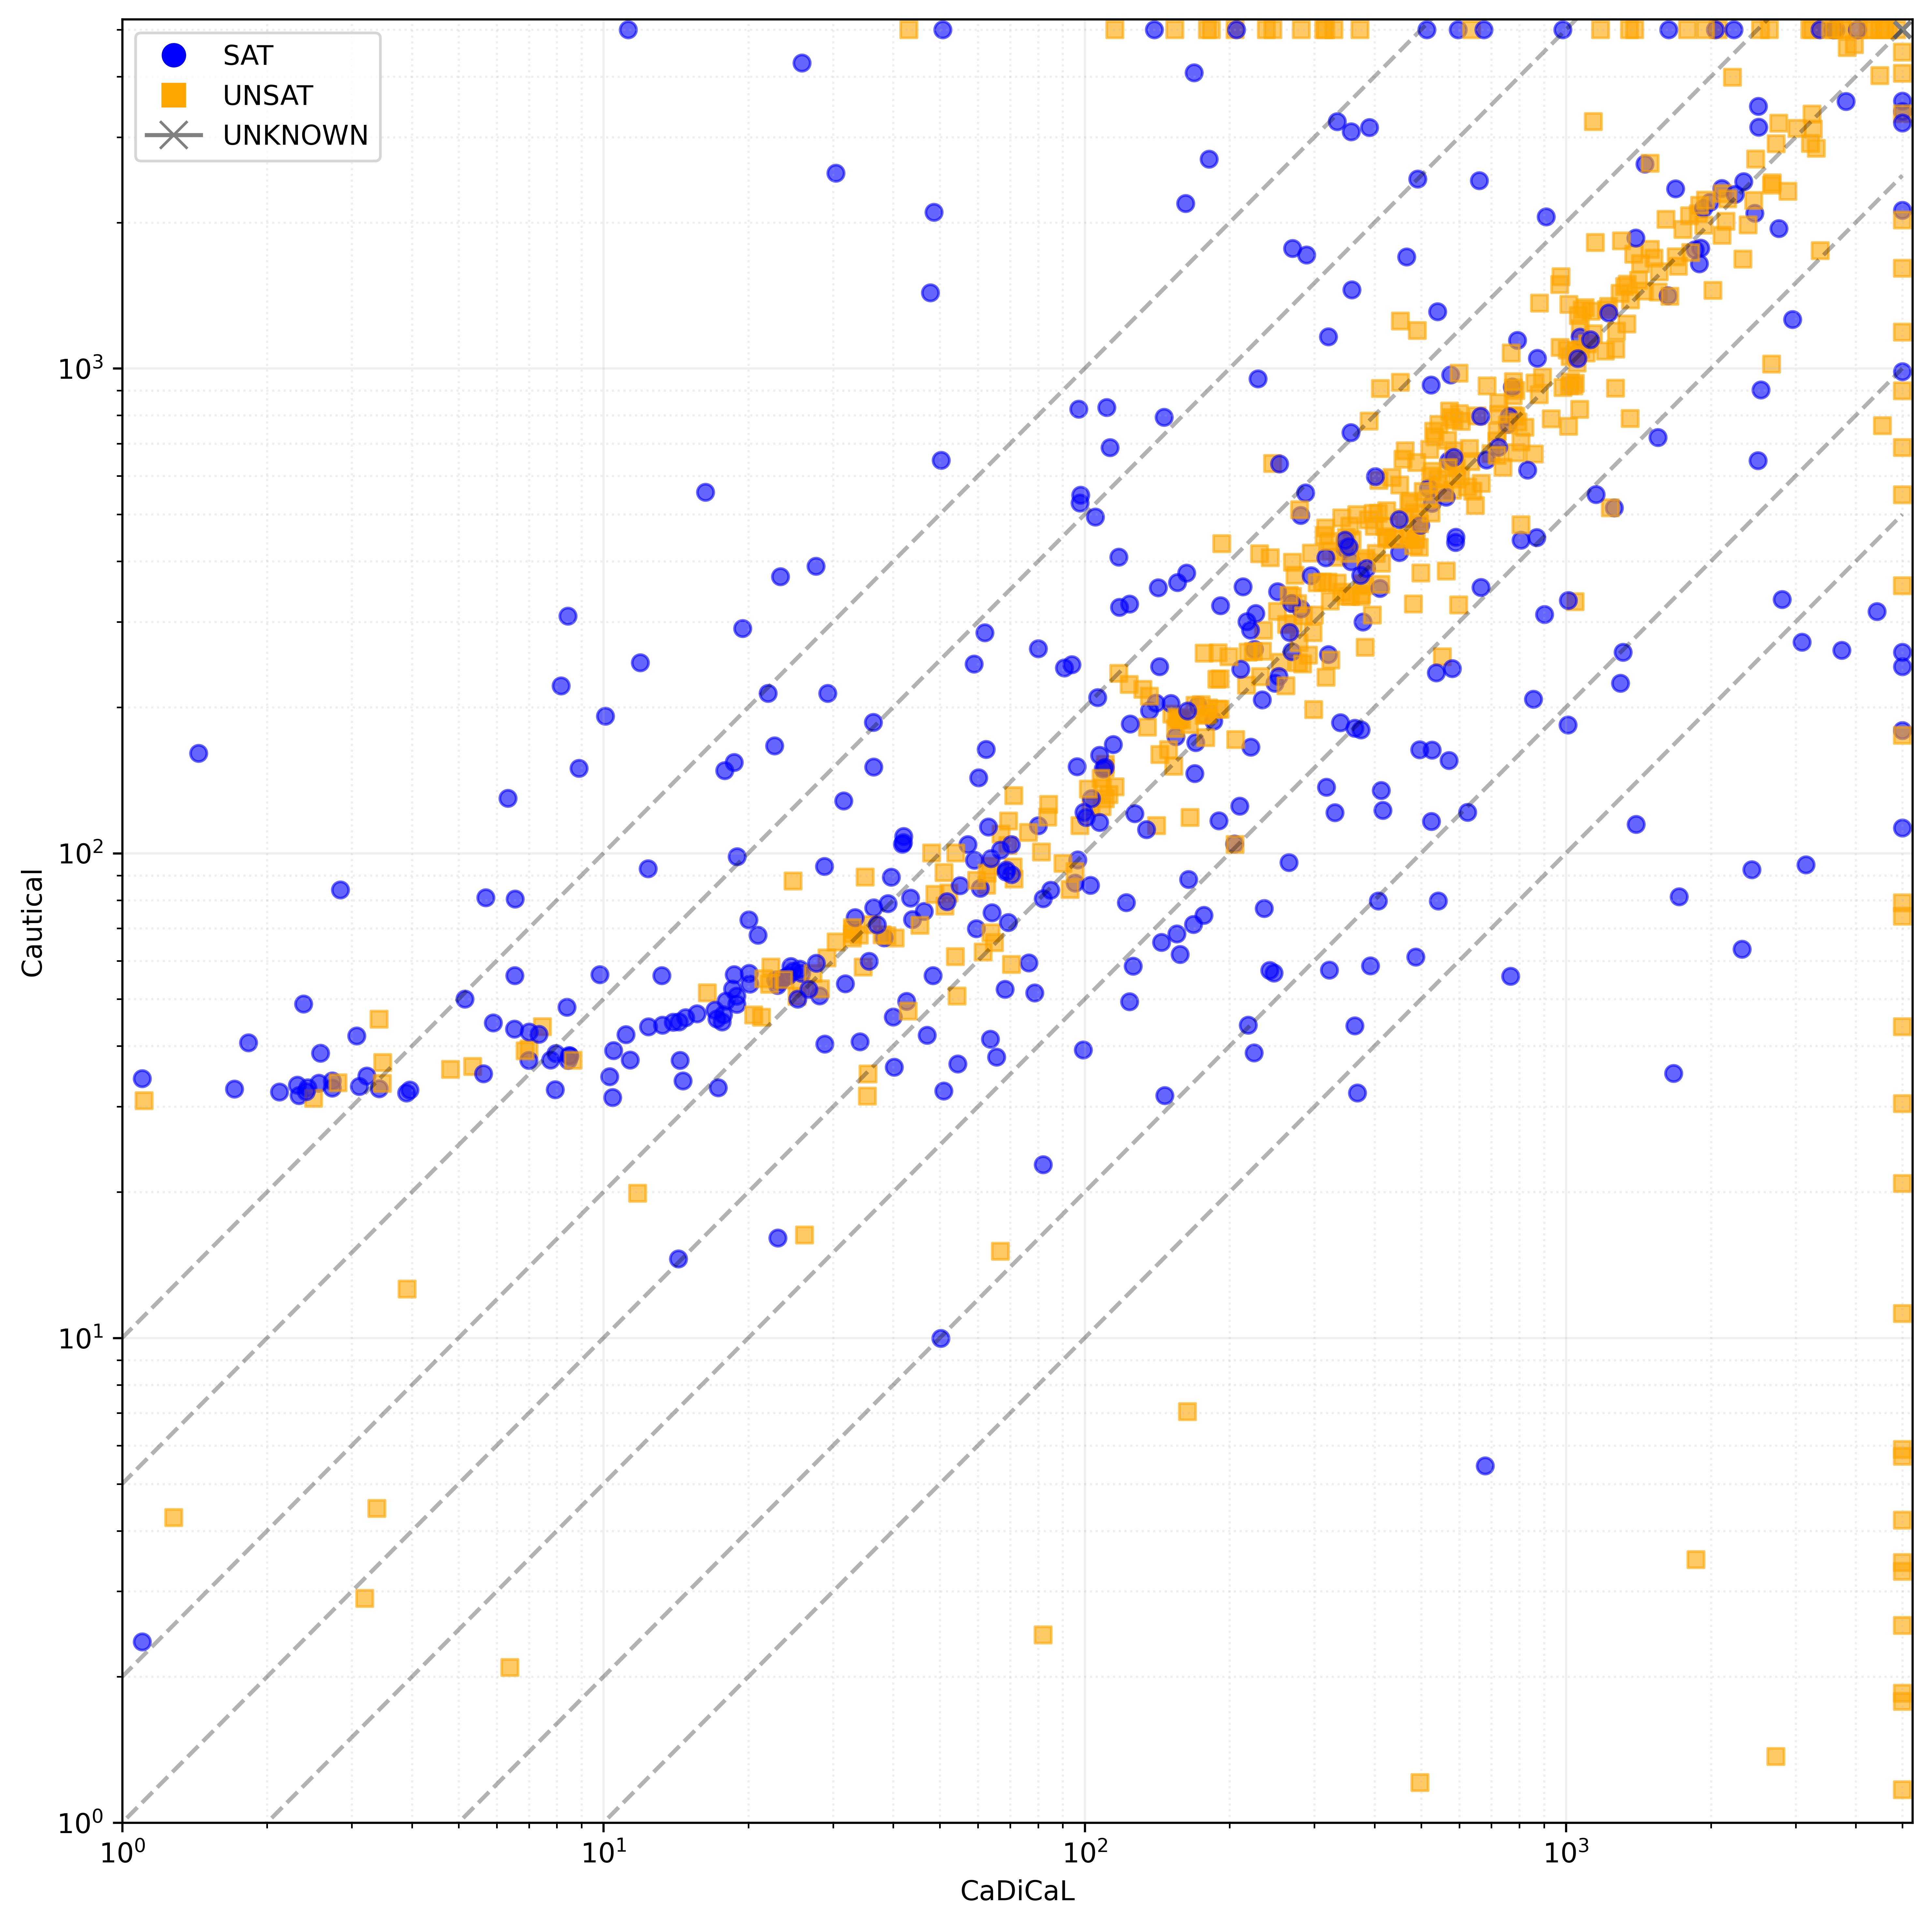
\includegraphics[width=\textwidth]{figs/cautical_vs_cadical_log.png}
        \caption{Comparison with \cadical}
        \label{fig:cautical-vs-cadical}
    \end{subfigure}
    \hspace{0.06\textwidth}
    \begin{subfigure}[t]{0.4\textwidth}
        \centering
        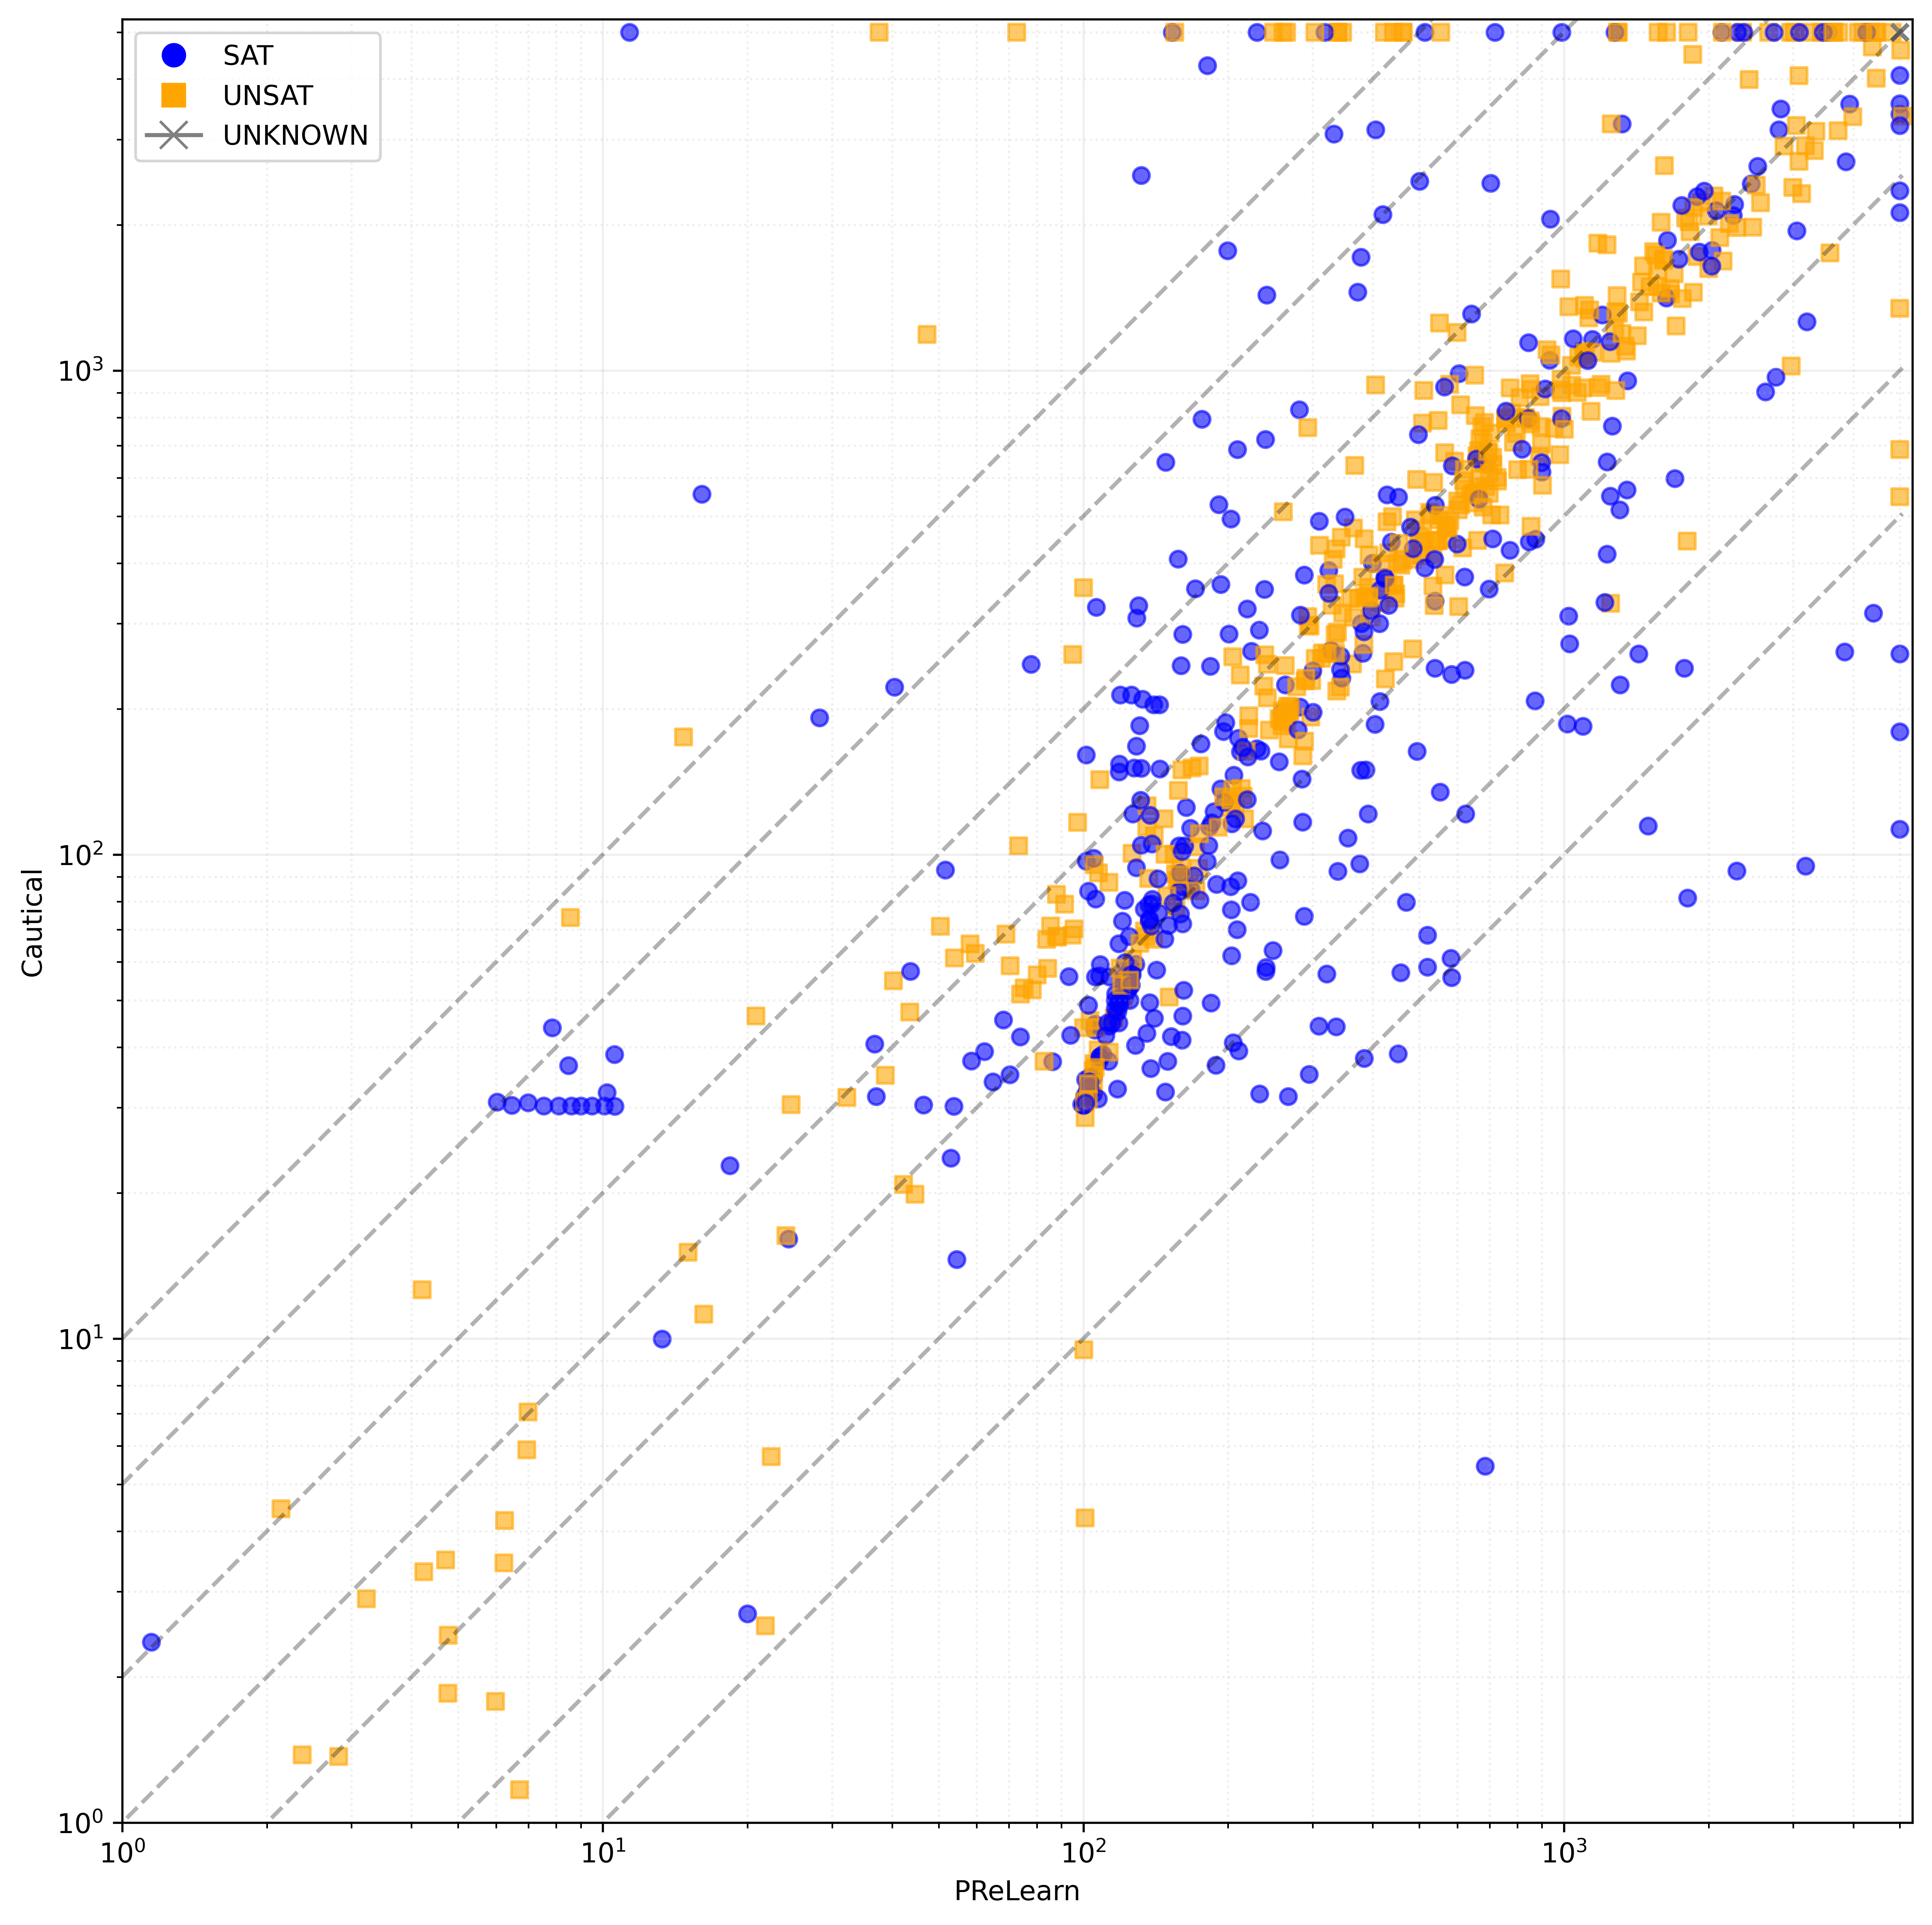
\includegraphics[width=\textwidth]{figs/cautical_vs_prelearn_log.png}
        \caption{Comparison with \prelearn}
        \label{fig:cautical-vs-prelearn}
    \end{subfigure}
    \caption{Performance comparison of \tool with other solvers}
    \label{fig:solver-comparison}
\end{figure*}

In \autoref{fig:solver-comparison}, we compare the performance of \tool with \cadical and \prelearn on the benchmarks from the annual Satisfiability competition from the years 2022, 2023, and 2024. \autoref{tab:solver-stats} shows the number of instances solved by each solver as well as the number of queries for which \prelearn and \cadical learn additional clauses, improve upon \cadical, and solve that \cadical does not solve.

The PAR-2 score is used to evaluate the performance of the solvers at the competition, it is the sum of the runtime on instances solved plus two times the timeout for each instance unsolved. On this dataset, \cadical has a PAR-score of 3970200.7 seconds, \prelearn has a PAR-score of 3791297.9 seconds, and \tool has a PAR-score of 4072090.4 seconds.

\begin{table}[ht]
    \centering
    \sisetup{table-format=3}        % remove if you are not using siunitx
    \begin{tabular}{lrrrr}
      \toprule
      & \multicolumn{2}{c}{0--10k} & \multicolumn{2}{c}{10k$+$} \\
      \cmidrule(lr){2-3} \cmidrule(lr){4-5}
      & SAT & UNSAT & SAT & UNSAT \\
      \midrule
      \cadical Solved      &  54 &  73 & 354 & 349 \\
      \midrule
      Total w/ \prelearn &  52 &  92 & 356 & 355 \\
      \prelearn learnt      &  43 &  75 & 216 & 203 \\
      Improved w/ \prelearn&  12 &  31 &  32 &  22 \\
      Only w/ \prelearn    &   1 &  19 &   6 &   9 \\
      \midrule
      Solved w/ \tool  &  52 &  87 & 349 & 327 \\
      \tool learnt     &  16 &  59 &  32 &  36 \\
      Improved w/ \tool&  23 &  33 &  87 &  78 \\
      Only w/ \tool    &   0 &  18 &   9 &   9 \\
      \bottomrule
    \end{tabular}
    \caption{Number of solved instances.}
    \label{tab:solver-stats}
  \end{table}

  

% \subsection{Analysis of heuristics}~\label{subsec:eval-heuristics}

% \subsection{Discussion of Benchmark Families}~\label{subsec:eval-discussion}
  \section{Conclusion and Future Work}~\label{sec:conclusion}


\pr clause learning is effective for learning short proofs for 
difficult problems. However, current \pr clause learning techniques require
an NP-hard check. We solve this by providing a technique that learns \pr clauses
in a linear time preprocessing step. We provide clause shrinking and filtering 
techniques to ensure that we learn useful \pr clauses.

Our implementation, \tool, provides short \pr proofs matching the best results for 
the pigeonhole principle. While prior work is only effective on specific pigeonhole
encodings, \tool finds these proofs even when the formula is scranfilized.

Additionally, \tool is effective on a number of benchmarks from the SAT competition,
including most of the families identified in \autoref{subsec:eval-discussion}.

In the future, we hope that \pr clause learning can find its way into the main branch
of popular SAT solver. We believe this work is an effective step in this direction.



%   \input{texs/back}
%   % \input{texs/method}
%   \input{texs/context}
%   \input{texs/shake}
%   \input{texs/eval}
%   \input{texs/related}
%   \input{texs/limit}
%   \input{texs/conclude}

  
  \newpage
  
  \clearpage
  
  \bibliographystyle{IEEEtran}
  \bibliography{base}

  % \appendix

  % \subsection{Pigeonhole Proof explained}~\label{app:pigeonhole}

\begin{figure*}[!t]
    \centering
    \begin{subfigure}[t]{0.23\textwidth}
    \centering
    \begin{tikzpicture}
      % Draw the 4×5 grid and name it "M"
      \matrix (M) [gridmatrix] {
        % row 1
        |[graycell]| & |[graycell]| & |[graycell]| & |[graycell]| \\
        % row 2
        |[redcell]|  & |[graycell]| & |[graycell]| & |[graycell]| \\
        % row 3
        |[graycell]| & |[graycell]| & |[graycell]| & |[graycell]| \\
        % row 4
        |[graycell]| & |[graycell]| & |[graycell]| & |[graycell]| \\
        % row 5
        |[graycell]| & |[graycell]| & |[graycell]| & |[graycell]| \\
      };

      % Column labels: attach ABOVE the north anchor of row 1 cells
      \foreach \c [count=\i from 1] in {$h_1$,$h_2$,$h_3$,$h_4$} {
        \node[anchor=south] at (M-1-\i.north) {\c};
      }

      % Row labels: attach LEFT of the west anchor of column 1 cells
      \foreach \r [count=\j from 1] in {$p_1$,$p_2$,$p_3$,$p_4$,$p_5$} {
        \node[anchor=east] at (M-\j-1.west) {\r};
      }
    \end{tikzpicture}
    \captionsetup{width=0.8\textwidth}  % override for this one only
    \caption{The first unit learned is of the form $x_{2, 1}$}~\label{subfig:pigeonhole-a}  
\end{subfigure}
\begin{subfigure}[t]{0.23\textwidth}
    \centering
    \begin{tikzpicture}
        % Draw the 4×5 grid and name it "M"
        \matrix (M) [gridmatrix] {
            % row 1
            |[graycell]| & |[graycell]| & |[graycell]| & |[graycell]| \\
            % row 2
            |[redcell]|  & |[graycell]| & |[graycell]| & |[graycell]| \\
            % row 3
            |[redcell]| & |[graycell]| & |[graycell]| & |[graycell]| \\
            % row 4
            |[redcell]| & |[graycell]| & |[graycell]| & |[graycell]| \\
            % row 5
            |[graycell]| & |[graycell]| & |[graycell]| & |[graycell]| \\
        };

        % Column labels: attach ABOVE the north anchor of row 1 cells
        \foreach \c [count=\i from 1] in {$h_1$,$h_2$,$h_3$,$h_4$} {
            \node[anchor=south] at (M-1-\i.north) {\c};
        }

        % Row labels: attach LEFT of the west anchor of column 1 cells
        \foreach \r [count=\j from 1] in {$p_1$,$p_2$,$p_3$,$p_4$,$p_5$} {
            \node[anchor=east] at (M-\j-1.west) {\r};
        }
    \end{tikzpicture}
    \captionsetup{width=0.8\textwidth}  % override for this one only
    \caption{In a similar fashion we then learn the units $\overline{x}_{3, 1}$ and $\overline{x}_{4, 1}$}~\label{subfig:pigeonhole-b} 
\end{subfigure}
\begin{subfigure}[t]{0.23\textwidth}
    \centering
    \begin{tikzpicture}
    % Draw the 4×5 grid and name it "M"
    \matrix (M) [gridmatrix] {
        % row 1
        |[graycell]| & |[redcell]| & |[redcell]| & |[redcell]| \\
        % row 2
        |[redcell]|  & |[graycell]| & |[graycell]| & |[graycell]| \\
        % row 3
        |[redcell]| & |[graycell]| & |[graycell]| & |[graycell]| \\
        % row 4
        |[redcell]| & |[graycell]| & |[graycell]| & |[graycell]| \\
        % row 5
        |[graycell]| & |[graycell]| & |[graycell]| & |[graycell]| \\
    };

    % Column labels: attach ABOVE the north anchor of row 1 cells
    \foreach \c [count=\i from 1] in {$h_1$,$h_2$,$h_3$,$h_4$} {
        \node[anchor=south] at (M-1-\i.north) {\c};
    }

    % Row labels: attach LEFT of the west anchor of column 1 cells
    \foreach \r [count=\j from 1] in {$p_1$,$p_2$,$p_3$,$p_4$,$p_5$} {
        \node[anchor=east] at (M-\j-1.west) {\r};
    }
    \end{tikzpicture}
    \captionsetup{width=0.8\textwidth}  % override for this one only
    \caption{By the symmetry argument, we learn units $\overline{x}_{1, 2}$, $\overline{x}_{1, 3}$, and $\overline{x}_{1, 4}$}~\label{subfig:pigeonhole-c}
\end{subfigure}
\begin{subfigure}[t]{0.23\textwidth}
    \centering
    \begin{tikzpicture}
    % Draw the 4×5 grid and name it "M"
    \matrix (M) [gridmatrix] {
        % row 1
        |[greencell]| & |[redcell]| & |[redcell]| & |[redcell]| \\
        % row 2
        |[redcell]|  & |[graycell]| & |[graycell]| & |[graycell]| \\
        % row 3
        |[redcell]| & |[graycell]| & |[graycell]| & |[graycell]| \\
        % row 4
        |[redcell]| & |[graycell]| & |[graycell]| & |[graycell]| \\
        % row 5
        |[redcell]| & |[graycell]| & |[graycell]| & |[graycell]| \\
    };

    % Column labels: attach ABOVE the north anchor of row 1 cells
    \foreach \c [count=\i from 1] in {$h_1$,$h_2$,$h_3$,$h_4$} {
        \node[anchor=south] at (M-1-\i.north) {\c};
    }

    % Row labels: attach LEFT of the west anchor of column 1 cells
    \foreach \r [count=\j from 1] in {$p_1$,$p_2$,$p_3$,$p_4$,$p_5$} {
        \node[anchor=east] at (M-\j-1.west) {\r};
    }
    \end{tikzpicture}
    \captionsetup{width=0.8\textwidth}  % override for this one only
    \caption{Constraint (1) gives $x_{1, 1}$, then constraint (2) gives $\overline{x}_{5, 1}$, completing the reduction to \ph{3}}~\label{subfig:pigeonhole-d}
\end{subfigure}


    \caption{Process for reducing \ph{4} to \ph{3}}
  \end{figure*}

We discuss the pigeonhole principle as a motivating example. The problem asks 
whether we can put $m$ pigeons in $n$ holes such that (1)~every pigeon is in a 
hole, and (2)~no hole contains more than one pigeon. This can be easily 
encoded as a SAT problem where variable $x_{i, j}$ represents putting the 
$i$-th pigeon into the $j$-th hole. We can translate constraint (1) as $\bigvee_{1 \leq j \leq n} x_{i, j}$ for each $1 \leq i \leq m$. We can also translate constraint (2) as $\overline{x}_{i, j} \lor \overline{x}_{k, j}$ for each $ 1 \leq i \neq k \leq m$ and $1 \leq j \leq n$.

We represent this diagrammatically as in \autoref{fig:pigeonhole}, where the rows are the pigeons and the columns are the holes. The cell in row $i$ and column $j$ represents the literal $x_{i, j}$, i.e. whether the $i$-th pigeon is in the $j$-th hole. If the $(i, j)$-th cell is green this represents $x_{i, j}$ is set to true and if it is red this represents $x_{i, j}$ is set to false. Thus, constraint (1) asks that each row has at least one green cell and constraint (2) asks that no two green cells share a column.

We will only consider the case where $m = n + 1$ which we denote \ph{n}. This is clearly unsatisfiable, however there are no polynomial-sized resolution proofs of \ph{n}~\cite{hakenpigeonhole}. There are $O(n^3)$ \pr proofs of the pigeonhole principle, but this is difficult to achieve in practice and requires specific techniques~\cite{prclauses}. We can learn these proofs, with a very low constant factor and little sensitivity to the encoding.


\subsection{Pigeonhole Setup}~\label{subsec:pigeonhole-setup}

Our technique makes a pair of decisions, propagates and then divides this assignment into a conditional and an autarky part, and finally shrinks the clause to derive a useful \pr clause.

While our technique does allow for decisions on negative literals, this is not useful for the Pigeonhole Principle. We first decide on some literal $i$. For ease, we assume that $i = x_{1, 1}$. This does not matter because of symmetry.

Notice that the set of literals we consider for $j$ are the \emph{touched literals}, i.e. those that are in a clause with $x_{1, 1}$ or any of the variables it propagates. By constraint (2), $x_{1, 1}$ propagates $\overline{x}_{k, 1}$ for $2 \leq k \leq n + 1$. But these literals will touch every literal in the formula via the clauses from constraint (1). 


\subsection{Solving the Pigeonhole Principle}~\label{subsec:solvingpigeonhole}

Below we describe three stages at which we learn useful clauses:


\subsubsection{Useful Binary Clauses}~\label{subec:usefulbinaryclauses} When learning a second variable $j= x_{2, 2}$, propagation gives us the literals $\overline{x}_{2, 1}, \dots \overline{x}_{n+1, 1}$ and $\overline{x}_{1, 2}, \overline{x}_{3, 2}, \dots \overline{x}_{n+1, 2}$. This can be divided into a autarky part $\alpha_a = x_{1, 1}, x_{2, 2}, \overline{x}_{1, 2}, \overline{x}_{2, 1}$ and a conditional part $\alpha_c = \overline{x}_{3, 1}, \ldots, \overline{x}_{n+1, 1}, \overline{x}_{3, 2}, \ldots, \overline{x}_{n+1, 2}$.

This can be shrunk to the clause $\overline{x}_{1, 2} \lor \overline{x}_{2, 1}$.
% todo : maybe say more about this shrinking

Then when considering the next assumption $j = x_{2, 3}$, we end up learning the clause $\overline{x}_{1, 3} \lor \overline{x}_{2, 1}$. This continues until we learn $\overline{x}_{1, n} \lor \overline{x}_{2, 1}$. Notice that have the clause $\overline{x}_{1, n} \lor \overline{x}_{2, 1}$ from constraint (2) and the clause $\bigwedge_{1 \leq j \leq n} x_{1, j}$ from constraint (1). These combined will yield the unit clause $\overline{x}_{2, 1}$ as shown in \autoref{subfig:pigeonhole-a}.

Similary, we can learn the unit clauses $\overline{x}_{3, 1}, \overline{x}_{4, 1}, \ldots, \overline{x}_{n, 1}$ as shown in \autoref{subfig:pigeonhole-b}.


\subsubsection{Useful Units} In the last row of learning, we get something even more useful. Starting with the assumption $j = x_{n+1, 2}$, we propagate the literals $\overline{x}_{n + 1, 1}$ and $\overline{x}_{1, 2}, \overline{x}_{2, 2}, \ldots, \overline{x}_{n, 2}$.  This can be divided into a autarky part $\alpha_a = x_{1, 1}, x_{n+1, 2}, \overline{x}_{1, 2}, \overline{x}_{n+1, 1}$ and a conditional part $\alpha_c = \overline{x}_{1, 2}, \ldots, \overline{x}_{n, 2}$.

Shrinking gives us just the unit clause $\overline{x}_{1, 2}$. Notice that if we had done this at the beginning, we would have also had $\overline{x}_{2, 1}, \ldots, \overline{x}_{n, 1}$ and thus shrinking would have given a binary clause.

In a similar manner, we also learn the units $\overline{x}_{2, 1}, \ldots, \overline{x}_{n, 1}$ as shown in \autoref{subfig:pigeonhole-c}.

\subsubsection{Final Simplifications} Finally, constraint (1) will allow us to learn the unit $x_{1, 1}$ and constraint (2) will imply the unit $x_{n+1, 1}$ as shown in \autoref{subfig:pigeonhole-d}. Thus, we have successfully reduced the \ph{n} to \ph{n-1}. Then we pick some other variable for $i$ (for instance $i = x_{2, 2}$) and repeat the process.

\subsection{Complexity Analysis}~\label{subsec:complexity analysis}

The complexity of this technique is $O(n^3)$ for the proof size. The time it takes to execute a proof step is linear in the size of a formula. Since the formula for pigeonhole has size $O(n^2)$, the total runtime is $O(n^5)$.

% \subsubsection{Proof Size}~\label{subsubsec:proof-size} 
We briefly remark on the constant factors in the proof size as they compare favorably to similar techniques. First, in the useful binary clause phase, we must learn $n-1$ binary clauses for each unit we learn. We end learning $n-1$ units, for a total of $(n-1)^2$ clauses (note the final binary clause and the unit clause can be learned together in a single step). Second, in the useful unit phase, we learn $n-1$ units, for a total of $n-1$ clauses. Third, in the final simplification phase, we learn 3 clauses. This gives a total of $n(n-1) + 3$ clauses to reduce \ph{n} to \ph{n-1}.

Thus, there needs to be 

  
  % \input{texs/appendix}
  
  \end{document}
  